\renewcommand\chapterillustration{./abertura-estatistica2}%Photo by 
\renewcommand\chapterwhat{Medidas de posição: média, mediana, moda e quartis. Medidas de dispersão:
desvio médio, variância, desvio padrão, amplitude amostral, distância entre quartis e
coeficiente de variação. Construção do desenho-esquemático (boxplot).} 
\renewcommand\chapterbecause{As medidas resumo (posição e dispersão) correspondem a uma síntese do conjunto de
dados observados e ao passo preliminar para fazer uma inferência estatística, ou seja, a
partir das informações obtidas na amostra, expandir nossas conclusões para a população.
Como as distribuições podem apresentar formas variadas é importante conhecer
diferentes tipos de medidas resumo, tanto de posição como de dispersão, para usar
medidas apropriadas em cada caso.} 
\chapter{Medidas de posição e dispersão}
\label{\detokenize{PE104:medidas-de-posicao-e-dispersao}}\label{\detokenize{PE104::doc}}

\mbox{}\thispagestyle{empty}\clearpage

\thispagestyle{empty}

\begin{center}
Projeto: LIVRO ABERTO DE MATEMÁTICA

\noindent \begin{tabular}{lcccr}

\includegraphics[scale=.15]{impa}& \quad\quad& 
\includegraphics[width=3cm]{logo} & \quad\quad& 
\includegraphics[scale=.24]{obmep} 
\end{tabular}
\end{center}

\vspace*{.3cm}

Cadastre-se como colaborador no site do projeto: \url{umlivroaberto.org}

Versão digital do capítulo:

\url{https://www.umlivroaberto.org/BookCloud/Volume_1/master/view/PE104.html}

% \begin{center}
%   \includegraphics[width=2cm]{canvas}
% \end{center}

\begin{tabular}{p{.15\textwidth}p{.7\textwidth}}
Título: & Medidas de Posição e Dispersão\\
\\
Ano/ Versão: & 2020 / versão 0.10 de 24 de junho de 2020\\
\\
Editora & Instituto Nacional de Matem\'atica Pura e Aplicada (IMPA-OS)\\
\\
Realização:& Olimp\'iada Brasileira de Matem\'atica das Escolas P\'ublicas (OBMEP)\\
\\
Produção:& Associação Livro Aberto\\
\\
Coordenação: & Fabio Simas e Augusto Teixeira (livroaberto@impa.br)\\
\\
  Autores: & Flávia Landim (coordenadora da equipe - UFRJ),\\
        & Nei Rocha (UFRJ),\\
             & Vanessa Matos (SEduc Angras dos Reis e Mesquita).\\
\\
Revisão: &  Cydara Ripoll  \\
		 &  Alexandre Silva \\
\\
Design: & Andreza Moreira (Tangentes Design) \\
\\
  Ilustrações: & --- \\ 
\\
Gráficos: & Beatriz Cabral e Tarso Caldas (Licenciandos da UNIRIO)\\
\\
  Capa: & Foto de Clement Chen, no Unsplash\\
  		& https://unsplash.com/photos/EvoIUzuW89s \\

\end{tabular}


\begin{figure}[b]
\begin{minipage}[l]{5cm}
\centering

{\large Licença:}

  
\includegraphics[width=3.5cm]{cc-by-sa1}
\end{minipage}\hfill
\begin{minipage}[c]{5cm}
\centering
{\large Desenvolvido por}


\includegraphics[width=2.5cm]{logo-associacao.jpg}
\end{minipage}
\begin{minipage}[r]{5cm}
\centering

{\large Patrocínio:}
  \vspace{1em}
  
\includegraphics[width=3.5cm]{itau}
\end{minipage}
\end{figure}

\mainmatter

\explore{medidas de posição}
\label{\detokenize{PE104-0:sec-explorando1}}\label{\detokenize{PE104-0:explorando-medidas-de-posicao}}\label{\detokenize{PE104-0::doc}}
No capítulo \textbf{\hyperref[est1-chap]{A Natureza Estatística}} trabalhamos com representações gráficas de conjuntos de dados com a finalidade de obter informações sobre estruturas da sua distribuição como estratégia para resumir os dados.
No exemplo dos resgistros de tempo deste capítulo, os 64 dados, no quadro a seguir

\begin{table}[H]
\centering
\caption{Registros de tempo de atividade do capítulo \textbf{\hyperref[est1-chap]{A Natureza Estatística}}}
\begin{tabu} to \textwidth{|c|c|c|c|c|c|c|c|}
\hline
\thead
A & B & C & D & E & F & G & H \\
\hline
3,03 & 4,37 & 5,04 & 5,73 & 4,03 & 5,37 & 6,04 & 6,74 \\ 
\hline
3,38 & 4,46 & 5,11 & 5,84 & 4,38 & 5,46 & 6,11 & 6,84 \\
\hline
3,60 & 4,55 & 5,19 & 5,95 & 4,60 & 5,55 & 6,19 & 6,96 \\ 
\hline
3,78 & 4,63 & 5,29 & 6,08 & 4,78 & 5,64 & 6,29 & 7,08 \\
\hline
3,92 & 4,71 & 5,36 & 6,23 & 4,92 & 5,72 & 6,36 & 7,23 \\
\hline
4,04 & 4,79 & 5,45 & 6,41 & 5,04 & 5,79 & 6,45 & 7,40 \\
\hline
4,16 & 4,87 & 5,54 & 6,62 & 5,16 & 5,87 & 6,54 & 7,63 \\
\hline
4,27 & 4,95 & 5,64 & 6,97 & 5,26 & 5,95 & 6,64 & 7,97 \\ 
\hline
\end{tabu}
\caption{64 registros de tempo de atividade do capítulo \textbf{\hyperref[est1-chap]{A Natureza Estatística}}}
\end{table}

foram organizados em 10 intervalos de classe, como mostra a tabela a seguir

\begin{table}[H]
\centering
\caption{Registros de tempo agrupados em intervalos de classe}
\label{\detokenize{PE104-0:id4}}
\begin{tabu} to \textwidth{|l|c|}
\hline
\thead
Intervalo de classe & Número de observações \\
\hline
{[} 3,0 ; 3,5 {[} & 2 \\
\hline
{[} 3,5 ; 4,0 {[} & 3 \\ 
\hline
{[} 4,0 ; 4,5 {[} & 7 \\
\hline
{[} 4,5 ; 5,0 {[} & 9 \\
\hline
{[} 5,0 ; 5,5 {[} & 11 \\
\hline
{[} 5,5 ; 6,0 {[} & 11 \\ 
\hline
{[} 6,0 ; 6,5 {[} & 9 \\ 
\hline
{[} 6,5 ; 7,0 {[} & 7 \\ 
\hline
{[} 7,0 ; 7,5 {[} & 3 \\
\hline
{[} 7,5 ; 8,0 {[} & 2 \\ 
\hline
\end{tabu}
\end{table}


que, por sua vez, foi usada para construir um gráfico, o histograma a seguir.

\begin{figure}[H]
\centering
\capstart

\begin{tikzpicture}
\begin{scope}[x=60, y = 15]
\matrix[column sep=0.5cm, row sep=0.5cm]{
	\draw (3,0) -- (8,0);
	\foreach \ye in {0,...,12}{
		\draw [help lines, lightgray] (2.5,\ye) -- (8.5,\ye);
		\node [left] at (2.5,\ye) {\ye} ;
	}
	\foreach \xl/ \xr/\y in {3.0/3.5/2,3.5/4.0/3,4.0/4.5/7,4.5/5.0/9,5.0/5.5/11,5.5/6.0/11,6.0/6.5/9,6.5/7.0/7,7.0/7.5/3,7.5/8.0/2}{
	\draw [fill=\currentcolor!80] (\xl,0) rectangle (\xr,\y);
	\node [right, rotate=270] at ($(\xl,0)!0.5!(\xr,0)$) {\xl  a \xr};
	}
	\filldraw[fill=gray] (5.5,0) -- (5.4,-3) -- (5.6,-3) -- cycle;
	\node [below] at (5.5,-3) {média};
\\};
\end{scope}
\end{tikzpicture}
\caption{Histograma dos registros de tempo}\label{\detokenize{PE104-0:fig-histograma-resposta}}\label{\detokenize{PE104-0:id5}}

\end{figure}

Observe que os 64 registros de tempo foram resumidos numa representação gráfica que revela o comportamento destes dados: registros de tempo entre 3,0 e 8,0, estrutura simétrica em torno da média dos resgistros de tempo que é 5,5.

O capítulo \textbf{Medidas de Posição e Dispersão} tem como objetivo responder, entre outras, as seguintes perguntas sobre um conjunto de dados quantitativos.
\begin{enumerate}
\item {} 
É possível encontrar valor(es) para resumir as observações? Qual(is) seria(m) este(s) valor(es)? Como encontrá-lo(s)?

\item {} 
Como medir se os dados estão “próximos” ou “afastados” uns dos outros?

\item {} 
Como você classifica a forma do gráfico construído para representar os dados?

\item {} 
Existe algum valor muito diferente dos demais? Como identificá-lo?

\end{enumerate}

Ao longo deste capítulo veremos como resumir a informação dos dados, usando apenas algumas medidas que caracterizam a distribuição em vez de usar toda a coleção de dados para descrevê-la. Por esta razão, tais medidas são chamadas medidas resumo.

Como as distribuições podem apresentar formas variadas é importante conhecer diferentes tipos de medidas resumo, tanto de posição como de dispersão, para usar medidas apropriadas em cada caso.

\phantomsection\label{\detokenize{PE104-0:ativ-notas-de-artes}}
\begin{task}{ notas de Artes}

Ao final de um trimestre, um professor de Artes registrou as seguintes notas de seus 35 alunos, listadas no quadro a seguir, em ordem crescente.

\begin{table}[H]
\centering
\begin{tabu} to \textwidth{|c|c|c|c|c|c|c|}
\hline
0,8 & 20 & 2,0 & 2,5 & 2,5 & 3,5 & 4,5 \\
\hline
5,0 & 5,4 & 5,5 & 5,5 & 5,5 & 6,0 & 6,0 \\
\hline
6,0 & 6,0 & 6,3 & 6,5 & 6,8 & 6,8 & 7,0 \\
\hline
7,0 & 7,0 & 7,0 & 7,3 & 7,3 & 7,5 & 7,5 \\
\hline
7,5 & 7,5 & 7,8 & 8,0 & 8,0 & 8,0 & 8,0 \\
\hline
\end{tabu}
\end{table}

Este professor verificou que a média da turma foi aproximadamente 5,93 (soma das notas \(S=207,5\)). Como a participação da turma foi muito boa ao longo do trimestre, o professor resolveu dar uma bonificação na nota de cada aluno desta turma, pensando em duas possibilidades:

\begin{enumerate}
\item {} 
acrescentar um ponto para cada aluno da turma;

\item {} 
aumentar em $20\%$ a nota de cada aluno da turma.



Na figura a seguir veja um histograma das notas sem a bonificação.  A tabela com os intervalos de classe considerados na construção do histograma é dada por

\begin{table}[H]
\centering
\caption{Distribuição de frequências das notas antes de bonificação}
\label{\detokenize{PE104-0:id6}}
\begin{tabu} to \textwidth{|l|c|}
\hline
\thead
Intervalo & Frequência absoluta \\
\hline
{[}0,2{[} & 1 \\
\hline
{[}2,4{[} & 5 \\
\hline
{[}4,6{[} & 6 \\ 
\hline
{[}6,8{]} & 23 \\
\hline
\end{tabu}
\end{table}

\begin{figure}[H]
\centering

\begin{tikzpicture}
\begin{scope}[x=10, y = 5]
\matrix[column sep=0.5cm, row sep=0.5cm]{
	\foreach \ye in {0,5,...,25}{
		\draw [help lines, lightgray] (-0,\ye) -- (10,\ye);
		\draw (0,\ye) -- (-0.4,\ye);
		\node [left] at (-0.4,\ye) {\ye} ;
	}
	\draw (-0.5,0) -- (10,0);
	\draw (0,0) -- (0,25);
	\foreach \xl/ \xr/\y in {0/2/1,2/4/5,4/6/6,6/8/23}{
	\draw [fill=\currentcolor!80] (\xl,0) rectangle (\xr,\y);
	%\node [right, rotate=270] at ($(\xl,0)!0.5!(\xr,0)$) {$\xl$  a $\xr$};
	}
	\foreach \x in {0,2,...,10}{
		\draw (\x,0) -- (\x,-0.4);
		\node [below] at (\x,-0.4) {\x};
	}
\node [rotate=90] at (-4,12.5) {Frequencia absoluta};
\node [below] at (5,-4) {Notas};
%	\filldraw[fill=destacado] (5.5,0) -- (5.4,-3) -- (5.6,-3) -- cycle;
%	\node [below] at (5.5,-3) {média};

\\};
\end{scope}

\end{tikzpicture}
\caption{Histograma das notas de Artes sem bonificação}\label{\detokenize{PE104-0:fig-histograma-notas-sem-bonificacao}}\label{\detokenize{PE104-0:id7}}\end{figure}

Os dois histogramas a seguir correspondem às notas, após usar cada uma das possibilidades consideradas pelo professor, mantendo quatro intervalos de classe, conforme as tabelas de frequências apresentadas.

\begin{figure}[H]
\centering
\begin{minipage}{0.4\textwidth}
\begin{tikzpicture}
\begin{scope}[x=10, y = 5]


	\foreach \ye in {0,5,...,25}{
		\draw [help lines, lightgray] (-0,\ye) -- (10,\ye);
		\draw (0,\ye) -- (-0.4,\ye);
		\node [left] at (-0.4,\ye) {\ye} ;
	}
	\draw (-0.5,0) -- (10,0);
	\draw (0,0) -- (0,25);
	\foreach \xl/ \xr/\y in {0/2/1,2/4/5,4/6/6,6/8/23}{
	\draw [fill=\currentcolor!80] (1.2*\xl,0) rectangle (1.2*\xr,\y);
	%\node [right, rotate=270] at ($(\xl,0)!0.5!(\xr,0)$) {$\xl$  a $\xr$};
	}
	\foreach \x in {0,2,...,10}{
		\draw (\x,0) -- (\x,-0.4);
		\node [below] at (\x,-0.4) {\x};
	}
\node [rotate=90] at (-4,12.5) {Frequencia absoluta};
\node [below] at (5,-4) {($\quad$)};
%	\filldraw[fill=destacado] (5.5,0) -- (5.4,-3) -- (5.6,-3) -- cycle;
%	\node [below] at (5.5,-3) {média};

\end{scope}
\end{tikzpicture}
\end{minipage}
\begin{minipage}{0.4\textwidth}
\begin{tikzpicture}
\begin{scope}[x=10, y = 5]



	\foreach \ye in {0,5,...,25}{
		\draw [help lines, lightgray] (-0,\ye) -- (10,\ye);
		\draw (0,\ye) -- (-0.4,\ye);
		\node [left] at (-0.4,\ye) {\ye} ;
	}
	\draw (-0.5,0) -- (10,0);
	\draw (0,0) -- (0,25);
	\foreach \xl/ \xr/\y in {0/2/1,2/4/5,4/6/6,6/8/23}{
	\draw [fill=\currentcolor!80] (\xl+1,0) rectangle (\xr+1,\y);
	%\node [right, rotate=270] at ($(\xl,0)!0.5!(\xr,0)$) {$\xl$  a $\xr$};
	}
	\foreach \x in {0,2,...,10}{
		\draw (\x,0) -- (\x,-0.4);
		\node [below] at (\x,-0.4) {\x};
	}
\node [rotate=90] at (-4,12.5) {Frequencia absoluta};
\node [below] at (5,-4) {($\quad$)};

%	\filldraw[fill=destacado] (5.5,0) -- (5.4,-3) -- (5.6,-3) -- cycle;
%	\node [below] at (5.5,-3) {média};

\end{scope}
\end{tikzpicture}
\end{minipage}

\caption{Histogramas das notas de Artes com bonificação}\label{\detokenize{PE104-0:fig-histogramas-notas-aleteradas}}\label{\detokenize{PE104-0:id8}}\end{figure}

\begin{table}[H]
\centering
\caption{Distribuição de frequências das notas após acréscimo de 1 ponto a cada nota}
\label{\detokenize{PE104-0:id9}}
\begin{tabu} to \textwidth{|l|c|}
\hline
\thead
Intervalo & Frequência absoluta \\
\hline
{[}1;3{[} & 1 \\
\hline
{[}3;5{[} & 5 \\
\hline
{[}5;7{[} & 6 \\
\hline
{[}7;9{]} & 23 \\
\hline
\end{tabu}
\end{table}
\begin{table}[H]
\centering
\caption{Distribuição de frequências das notas após aumento de 20\% sobre a nota}
\label{\detokenize{PE104-0:id10}}
\begin{tabu} to \textwidth{|l|c|}
\hline
\thead
Intervalo & Frequência absoluta \\
\hline
{[}0 ; 2,4{[} & 1 \\
\hline
{[}2,4 ; 4,8{[} & 5 \\
\hline
{[}4,8 ; 7,2{[} & 6 \\ 
\hline
{[}7,2 ; 9,6{]} & 23 \\
\hline
\end{tabu}
\end{table}

\item {} 
Compare os histogramas das notas com bonificação com o histograma original. O que mudou em cada um deles em relação ao original?

\item {} 
Considerando os \hyperref[\detokenize{PE104-0:fig-histogramas-notas-aleteradas}]{Histogramas das notas de Artes com bonificação}, identifique qual deles corresponde ao  acréscimo de 1,0 ponto, assinalando (a) e qual deles corresponde ao aumento de 20\% das notas originais, assinalando (b).

\item {} 
Dada a informação inicial de que a média da turma foi 5,93, de quanto será a média se o professor acrescentar um ponto a cada aluno? E se ele aumentar em 20\% a nota de cada aluno?

\item {} 
Se você fosse um aluno desta turma, que possibilidade de bonificação você escolheria? Para que notas é melhor cada uma das estratégias?

\end{enumerate}
\end{task}


\phantomsection\label{\detokenize{PE104-0:ativ-maratona-de-ny}}
\begin{task}{ a maratona}

A maratona é uma prova de atletismo que consiste em correr uma distância de 42,195 km. Pelas suas características, este tipo de prova é realizada nas ruas de uma grande cidade ou na estrada. As principais cidades do mundo realizam um destes eventos anualmente, recebendo milhares de atletas profissionais e amadores que encaram o desafio e almejam finalizar a corrida ou melhorar o próprio tempo do passado.

Uma das mais famosas é a Maratona da Cidade de Nova Iorque, nos Estados Unidos. Veja na figura \hyperref[\detokenize{PE104-0:fig-maratona-ny}]{Corredores participando da Maratona de Nova York, Wikipedia} realização de uma maratona em Nova Iorque. Com mais de 50.000 participantes cada ano, é um dos principais eventos do atletismo mundial, junto com as maratonas de Chicago, Londres, Boston, Berlim e Tóquio.

\begin{figure}[H]
\centering

\includegraphics[width=200bp]{{New_York_marathon_Verrazano_bridge}.jpg}
\caption{Corredores participando da Maratona de \emph{Nova York}, 
\href{https://commons.wikimedia.org/wiki/File:New\_York\_marathon\_Verrazano\_bridge.jpg}{Wikipedia}}
\label{\detokenize{PE104-0:fig-maratona-ny}}
\label{\detokenize{PE104-0:id11}}
\end{figure}

Os resultados do evento são divididos nas categorias de homens e mulheres, além disso, no evento participam cadeirantes e pessoas usando triciclos de mão (\emph{handcycle}), categorias cujos resultados são premiados e publicados separadamente. Qual das categorias você acha que terá os melhores resultados na maratona? Em quanto tempo você acha que uma pessoa percorre os 42,195 km? O que você acha ser mais rápido: correr em cadeira de rodas ou em triciclo de mão?

\phantomsection\label{\detokenize{PE104-0:handcycle}}
\begin{figure}[H]
\centering
\includegraphics[width=200bp]{{Handcycle_in_Richmond_Park_-_geograph.org.uk_-_1315077}.jpg}
\label{\detokenize{PE104-0:handcycle}}
\end{figure}

A seguir analisaremos os tempos de corrida das 100 melhores atletas na categoria de Mulheres da Maratona de Nova York do ano 2017, dados disponíveis no \href{http://results.nyrr.org/event/M2017/finishers}{site oficial da competição}.

Observe no quadro a seguir, que os tempos já estão ordenados do menor para o maior e que para identificar o tempo da quadragésima sétima chegada, basta tomar a interseção da linha 7 com a coluna +40 para obter o tempo 2:55:36

\begin{table}[H]
\centering
\caption{100 melhores tempos de finalização da Maratona de Nova Iorque 2017 para mulheres (hora:minuto:segundo)}
\setlength\tabcolsep{2.5pt}
\label{\detokenize{PE104-0:id12}}
\begin{tabu} to \textwidth{|c|r|r|r|r|r|r|r|r|r|r|}
\hline
\thead
& +0 & +10 & +20 & +30 & +40 & +50 & +60 & +70 & +80 & +90 \\
\hline
1 & 2:26:53 & 2:32:01 & 2:42:52 & 2:49:44 & 2:53:59 & 2:56:58 & 2:58:35 & 2:59:36 & 3:01:24 & 3:03:43 \\
\hline
2 & 2:27:54 & 2:32:09 & 2:44:26 & 2:49:59 & 2:54:42 & 2:57:05 & 2:58:36 & 2:59:41 & 3:01:26 & 3:03:46 \\
\hline
3 & 2:28:08 & 2:33:18 & 2:44:48 & 2:50:04 & 2:54:52 & 2:57:10 & 2:58:50 & 2:59:43 & 3:01:28 & 3:04:02 \\
\hline
4 & 2:29:36 & 2:34:10 & 2:45:20 & 2:50:05 & 2:55:04 & 2:57:40 & 2:58:52 & 2:59:46 & 3:01:44 & 3:04:04 \\
\hline
5 & 2:29:39 & 2:34:23 & 2:45:52 & 2:51:11 & 2:55:25 & 2:57:49 & 2:58:56 & 2:59:51 & 3:02:09 & 3:04:17 \\
\hline
6 & 2:29:39 & 2:36:38 & 2:46:45 & 2:53:01 & 2:55:34 & 2:57:49 & 2:59:01 & 2:59:56 & 3:02:15 & 3:04:26 \\
\hline
7 & 2:29:41 & 2:37:22 & 2:47:04 & 2:53:02 & 2:55:36 & 2:57:50 & 2:59:03 & 3:00:02 & 3:02:39 & 3:04:42 \\
\hline
8 & 2:29:56 & 2:37:33 & 2:47:30 & 2:53:02 & 2:55:39 & 2:58:08 & 2:59:10 & 3:00:05 & 3:02:41 & 3:04:49 \\
\hline
9 & 2:31:21 & 2:39:01 & 2:47:35 & 2:53:19 & 2:56:47 & 2:58:23 & 2:59:16 & 3:00:49 & 3:02:56 & 3:04:58 \\
\hline
10 & 2:31:44 & 2:40:09 & 2:49:37 & 2:53:38 & 2:56:57 & 2:58:26 & 2:59:23 & 3:01:18 & 3:03:32 & 3:05:09 \\
\hline
\end{tabu}
\end{table}


\begin{reflection}
\begin{itemize}
\item {} 
Como você calcularia a média de valores em horas, minutos e segundos,  como os da tabela?

\item {} 
Como você construiria um histograma com estes dados? Como você definiria os limites dos intervalos? (Consulte a atividade \hyperref[est1-ativ-9]{Construção do Histrograma} do capítulo \textbf{\hyperref[est1-chap]{A Natureza Estatística}} em caso de dúvida.)

\item {} 
Qual o maior tempo em que uma corredora deveria completar a maratona para ficar entre as 25 primeiras? E entre as 50 primeiras?

\end{itemize}
\end{reflection}

Para calcular a média destes dados é conveniente reduzi-los a uma única unidade de medida, pois, caso contrário, seria necessário calcular três médias e, ainda fazer conversões apropriadas para obter a resposta em hora:minuto:segundo. Convertendo todos os tempos para horas, obtemos o seguinte quadro de tempos.

\begin{table}[H]
\centering
\begin{tabu} to \textwidth{|c|r|r|r|r|r|r|r|r|r|r|}
\hline
\thead
& +0 & +10 & +20 & +30 & +40 & +50 & +60 & +70 & +80 & +90 \\
\hline
1 & 2,448 & 2,534 & 2,714 & 2,829 & 2,900 & 2,949 & 2,976 & 2,993 & 3,023 & 3,062 \\
\hline
2 & 2,465 & 2,536 & 2,741 & 2,833 & 2,912 & 2,951 & 2,977 & 2,995 & 3,024 & 3,063 \\ 
\hline
3 & 2,469 & 2,555 & 2,747 & 2,834 & 2,914 & 2,953 & 2,981 & 2,995 & 3,024 & 3,067 \\
\hline
4 & 2,493 & 2,569 & 2,756 & 2,835 & 2,918 & 2,961 & 2,981 & 2,996 & 3,029 & 3,068 \\
\hline
5 & 2,494 & 2,573 & 2,764 & 2,853 & 2,924 & 2,964 & 2,982 & 2,998 & 3,036 & 3,071 \\
\hline
6 & 2,494 & 2,611 & 2,779 & 2,884 & 2,926 & 2,964 & 2,984 & 2,999 & 3,038 & 3,074 \\
\hline
7 & 2,495 & 2,623 & 2,784 & 2,884 & 2,927 & 2,964 & 2,984 & 3,001 & 3,044 & 3,078 \\
\hline
8 & 2,499 & 2,626 & 2,792 & 2,884 & 2,928 & 2,969 & 2,986 & 3,001 & 3,045 & 3,080 \\
\hline
9 & 2,523 & 2,650 & 2,793 & 2,889 & 2,946 & 2,973 & 2,988 & 3,014 & 3,049 & 3,083 \\
\hline
10 & 2,529 & 2,669 & 2,827 & 2,894 & 2,949 & 2,974 & 2,990 & 3,022 & 3,059 & 3,086 \\
\hline
\end{tabu}
\end{table}

\begin{enumerate}
\item {} 
Construa um histograma dos dados convertidos para horas, completando a tabela a seguir, que indica os intervalos de classe.

\end{enumerate}

\begin{table}[H]
\centering
\begin{tabu} to \textwidth{|l|c|}
\hline
\thead
Intervalo & Frequência \\
\hline
{[}2,4480 ; 2,5118{[} & \\
\hline
{[}2,5118 ; 2,5756{[} & \\
\hline
{[}2,5756 ; 2,6394{[} & \\
\hline
{[}2,6394 ; 2,7032{[} & \\
\hline
{[}2,7032 ; 2,7670{[} & \\
\hline
{[}2,7670 ; 2,8308{[} & \\
\hline
{[}2,8308 ; 2,8946{[} & \\
\hline
{[}2,8946 ; 2,9584{[} & \\
\hline
{[}2,9584 ; 3,0222{[} & \\
\hline
{[}3,0222 ; 3,0860{[} & \\
\hline
\end{tabu}
\end{table}

\begin{figure}[H]
\centering
\capstart

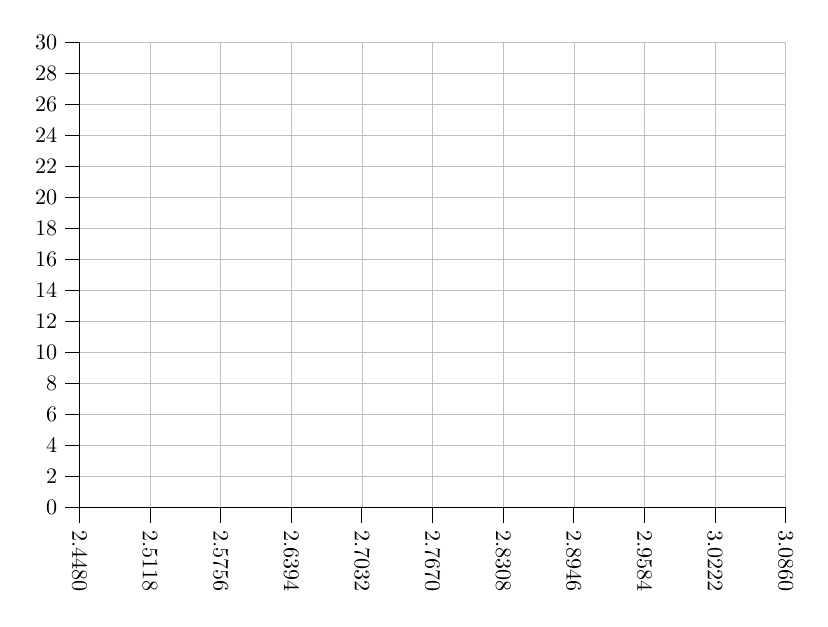
\begin{tikzpicture}[scale=.8, every node/.style={scale=.8}]
\begin{scope}[x=500, y = 7]
	\foreach \ye in {0,2,...,30}{
		\draw [help lines, lightgray] (2.4480,\ye) -- (3.0860,\ye);
		\draw (2.4480,\ye) -- (2.435,\ye);
		\node [left] at (2.435,\ye) {\ye} ;
	}
	\foreach \xe in {2.4480,2.5118,2.5756,2.6394,2.7032,2.7670,2.8308,2.8946,2.9584,3.0222,3.0860}{
		\draw [help lines, lightgray] (\xe,0) -- (\xe,30);
		\draw (\xe,0) -- (\xe,-1);
		\node [right,rotate=-90] at (\xe,-1) {\xe} ;
	}
	\draw (2.4480,30) -- (2.4480,0) -- (3.0860,0);
%	\filldraw[fill=destacado] (5.5,0) -- (5.4,-3) -- (5.6,-3) -- cycle;
%	\node [below] at (5.5,-3) {média};
\end{scope}

\end{tikzpicture}\caption{Eixos para a construção do histograma}\label{\detokenize{PE104-0:hist-maratona-mulheres}}\label{\detokenize{PE104-0:id15}}\end{figure}
\begin{enumerate}
\setcounter{enumi}{1}
\item {} 
Que características da distribuição dos 100 melhores tempos para mulheres podem ser destacadas, analisando-se o histograma construído?

\item {} 
Calcule o tempo médio dos 100 melhores tempos das corredoras, sabendo que a soma dos tempos é 286,978 horas. Localize o valor encontrado no eixo horizontal do histograma. Em que posição ficaria uma corredora cujo tempo no qual completou a maratona é igual ao tempo médio calculado neste item?

\item {} 
Trace linhas verticais no histograma de modo a separar as classificações em 4 grupos: uma linha vertical que identifica o 25$^{\circ}$ lugar, separando os 25 primeiros colocados dos demais; outra, que identifica a 50$^{\text{a}}$ classificação e, por fim, uma que marca o 75$^{\circ}$ tempo na classificação geral.

As marcações dos tempos das 25$^{\text{a}}$, 50$^{\text{a}}$ e 75$^{\text{a}}$ posições neste conjunto de 100 observações são chamadas de quartis da distribuição, este conceito será formalizado adiante.

\item {} 
Considerando as marcações realizadas no item anterior, determine aproximadamente as medidas das áreas contando os retângulos da grade do histograma correspondentes aos seguintes intervalos de tempo
\begin{enumerate}
\item {} 
1$^{\circ}$ até o 25$^{\circ}$;

\item {} 
25$^{\circ}$ até o 50$^{\circ}$;

\item {} 
50$^{\circ}$ até o 75$^{\circ}$;

\item {} 
75$^{\circ}$ até o 100$^{\circ}$;

\end{enumerate}

e compare-as.

\item {} 
Calcule os comprimentos dos intervalos de tempo determinados pela proposta de divisão no item (d) e compare-os.



\begin{table}[H]
\centering
\begin{tabu} to \textwidth{|c|c|}
\hline
\thead
Intervalo & Comprimento \\
\hline
1$^{\circ}$ a 25$^{\circ}$ & \\
\hline
25$^{\circ}$ a 50$^{\circ}$ & \\
\hline
50$^{\circ}$ a 75$^{\circ}$ & \\
\hline
75$^{\circ}$ a 100$^{\circ}$ & \\
\hline
\end{tabu}
\end{table}

\item {} 
O valor obtido para o tempo médio coincide com alguma das outras marcas feitas no histograma?

\item {} 
Observe que o tempo médio dos 100 melhores tempos para mulheres e o tempo da  corredora que chegou em 50o. lugar são diferentes. Qual deles você escolheria como medida resumo destes dados? Por quê?

\end{enumerate}
\end{task}


\arrange{  medidas de posição}
\label{\detokenize{PE104-1:sec-organizando1}}\label{\detokenize{PE104-1::doc}}\label{\detokenize{PE104-1:organizando-as-ideias-medidas-de-posicao}}
Medidas de Posição, como o próprio termo indica, visam a resumir um conjunto de dados em geral numa única medida em algum lugar geométrico entre os extremos observados do conjunto (mínimo e máximo). Veja na figura a seguir, as marcações da média e da mediana das notas de Artes sem bonificação.

\begin{figure}[H]
\centering
\capstart

\begin{tikzpicture}
\begin{scope}[x=15, y = 5]
	\foreach \ye in {0,5,...,25}{
		\draw [help lines, lightgray] (-0,\ye) -- (10,\ye);
		\draw (0,\ye) -- (-0.4,\ye);
		\node [left] at (-0.4,\ye) {\ye} ;
	}
	\draw (-0.5,0) -- (10,0);
	\draw (0,0) -- (0,25);
	\foreach \xl/ \xr/\y in {0/2/1,2/4/5,4/6/6,6/8/23}{
	\draw [ thick, fill=\currentcolor!80] (\xl,0) rectangle (\xr,\y);
	%\node [right, rotate=270] at ($(\xl,0)!0.5!(\xr,0)$) {$\xl$  a $\xr$};
	}
	\foreach \x in {0,2,...,10}{
		\draw (\x,0) -- (\x,-0.4);
		\node [below] at (\x,-0.4) {\x};
	}
\node at (5, 30) {Histograma das notas de Artes};
\node [rotate=90] at (-3,12.5) {Frequencia absoluta};
\node [below] at (5,-4) {Notas};
\draw [color=destacado, very thick, dashed] (5.93,-0.4) -- (5.93,27);
\node [left, color=destacado] at (5.93,27) {média};
\draw [color=atento, very thick, dashed] (6.5,-0.4) -- (6.5,27);
\node [right, color=atento] at (6.5,27) {mediana};
%	\filldraw[fill=destacado] (5.5,0) -- (5.4,-3) -- (5.6,-3) -- cycle;
%	\node [below] at (5.5,-3) {média};
\end{scope}

\end{tikzpicture}
\caption{Média e mediana assinaladas no Histograma de das notas de Artes}\label{\detokenize{PE104-1:fig-coloque-aqui-o-nome}}\label{\detokenize{PE104-1:id6}}\end{figure}

Só é possível obter medidas como a média e a mediana, se nossas observações são de natureza quantitativa, pois, como vimos no capítulo
\textbf{\hyperref[est1-chap]{A Natureza Estatística}}, as variáveis qualitativas estão no domínio da frequência apenas, ou seja, só podemos contar quantas observações ocorrem em cada categoria da variável qualitativa, mas não podemos operar matematicamente com as categorias em si. Por exemplo, na atividade Prática de Atividades Físicas deste capítulo, trabalhamos com a variável modalidade do esporte praticado. As modalidades correspondem à “Futebol”, “Caminhada”, “Fitness”, etc. Observe que são respostas não numéricas e, por isso, não podemos calcular uma média e não existe uma relação de ordem natural das respostas. Apenas podemos ordenar as respostas pela frequência na qual elas ocorreram.

As principais medidas de posição usadas na Estatística são a média, a mediana, a moda e os quartis da distribuição. Outras medidas de posição existem, mas não são tão usuais.

Definiremos a seguir as principais medidas que buscam de alguma forma resumir a informação do conjunto.

Para definir várias medidas a serem estudadas neste capítulo vamos adotar a seguinte notação.

\begin{example}{Idade de pessoas que tomaram a vacina da febre amarela}

Suponha que na primeira segunda-feira do mês de março de 2018, um Posto de Saúde tenha registrado as idades (em anos completos) das seis primeiras pessoas que chegaram para tomar a vacina da febre amarela e, os registros, obtidos foram \(\{55, 22, 30, 14, 25, 40\}\). Neste exemplo dizemos que o número de observações, denotado por \(n\), é \(6\) e que as observações são dadas por \(x_1=55\), \(x_2=22\), \(x_3=30\), \(x_4=14\), \(x_5=25\) e \(x_6=40\).

De um modo geral, sejam \(x_1,x_2, \cdots, x_n\) , os \(n\) valores observados de uma variável quantitativa tal que

\(x_1\) é o primeiro valor observado; \(x_2\) é o segundo valor observado; e, assim por diante, tal que \(x_n\) é o último valor observado.

Os valores observados não ocorrem necessariamente de forma ordenada do menor para o maior. Neste exemplo, das idades das três primeiras pessoas que chegaram para tomar a vacina no Posto de Saúde foram \(x_1=55\), \(x_2=22\) e \(x_3=30\) de modo que \(x_1>x_2\) e \(x_2<x_3\).

Para definir a mediana, será útil usar uma notação para representar os dados ordenados.

Sejam \(x_{(1)}\) o menor valor do conjunto \(\{ x_1,x_2,...,x_n\}\); \(x_{(2)}\), o segundo menor valor do conjunto \(\{ x_1,x_2,...,x_n\}\); e assim sucessivamente até \(x_{(n)}\), o maior valor do conjunto \(\{ x_1,x_2,...,x_n\}\).

Desse modo,
\(x_{(1)}\leq x_{(2)}\leq \cdots\leq x_{(n)}\) são os valores ordenados do conjunto \(\{ x_1,x_2,...,x_n\}\).

No exemplo das idades das seis primeiras pessoas que chegaram para tomar a vacina no Posto de Saúde, os registros obtidos foram \(\{55, 22, 30, 14, 25, 40\}\) tal que

$$x_1=55, x_2=22, x_3=30, x_4=14, x_5=25 \text{ e } x_6=40$$

e

$$x_{(1)}=14, x_{(2)}=22, x_{(3)}=25, x_{(4)}=30, x_{(5)}=40 \text{ e } x_{(6)}=55$$

\end{example}

A letra maiúscula sigma \(\left (\Sigma\right )\) é usada para denotar somatório, simplificando algumas fórmulas. Por exemplo,
\begin{equation*}
\begin{split}\sum^n_{i=1} x_i=x_1+x_2+\cdots +x_n\end{split}
\end{equation*}
e
\begin{equation*}
\begin{split}\sum^n_{i=1} x^2_i=x^2_1+x^2_2+\cdots +x^2_n\end{split}
\end{equation*}
Observe que neste exemplo, das idades das seis primeiras pessoas que chegaram para tomar a vacina no Posto de Saúde,
\begin{equation*}
\begin{split}\sum^6_{i=1}x_i=x_1+x_2+x_3+x_4+x_5+x_6=\\
55 + 22 + 30 + 14 + 25 + 40 = 186\end{split}
\end{equation*}
e
\begin{equation*}
\begin{split}\sum^n_{i=1} x^2_i=x^2_1+x^2_2+x^2_3+x^2_4+x^2_5 +x^2_6=\\
55^2+ 22^2+ 30^2+ 14^2+ 25^2+  40^2=6.830\end{split}
\end{equation*}
\textbf{Média}

A definição de média de um conjunto de dados quantitativos já é conhecida desde o Ensino Fundamental e, consiste na soma dos valores do conjunto dividida pelo número de observações. No exemplo das idades das seis primeiras pessoas que chegaram para tomar a vacina no Posto de Saúde, a soma das idades é 186 tal que a média será dada por \(\frac{186}{6}=31\) anos.

De modo mais geral, considere um conjunto contendo \(n\) valores de uma variável quantitativa representado por \(\{x_1,x_2,\cdots,x_n\}\).
A \index{média}média deste conjunto, denotada por \(\bar{x}\),  é definida por
\begin{equation*}
\begin{split}\bar{x}=\frac{\sum^n_{i=1}x_i}{n}=\frac{x_1+x_2+\cdots x_n}{n}\end{split}
\end{equation*}
Observe que a média pode substituir todas as observações sem alterar a  soma dos valores, isto é,
\begin{equation*}
\begin{split}x_1+x_2+\cdots+x_n=\bar{x}+\bar{x}+\cdots+\bar{x} = n\cdot \bar{x}\end{split}
\end{equation*}
fornecendo a expressão que define a média, denotada por \(\bar{x}\) .

Esta é justamente a ideia por trás da definição de qualquer média: uma medida que de alguma forma representa o conjunto de dados, segundo uma formulação, e se situa entre os extremos das observações. É claro que, em geral, haverá valores diferentes no conjunto e, neste caso, a média será um valor pertencente ao intervalo de variação dos valores neste conjunto e não necessariamente, um valor que tenha sido observado.

No exemplo das idades das seis primeiras pessoas que chegaram para tomar a vacina no Posto de Saúde a média é 31 anos, porém não se observou uma idade igual a 31 anos.

Você já calculou a média dos dados das duas primeiras atividades, a saber, \hyperref[\detokenize{PE104-0:ativ-notas-de-artes}]{Notas de Arte} e \hyperref[\detokenize{PE104-0:ativ-maratona-de-ny}]{A Maratona}. Identifique nos histogramas correspondentes a posição em que estas médias ficaram.

\textbf{Média para dados agrupados}

Quando os dados disponíveis estão agrupados em intervalos de classe,  não é possível calcular a soma total exata dos dados. Neste caso, usamos uma aproximação para o cálculo da média como mostra o exemplo a seguir.

Suponha que um coordenador tenha tido acesso apenas ao \hyperref[\detokenize{PE104-0:fig-histograma-notas-sem-bonificacao}]{Histograma das notas de Artes sem bonificação}, sem conhecer as notas separadamente.  Como este coordenador poderia calcular a média da turma, considerando as notas antes da bonificação?

Temos a seguinte distribuição de frequências das notas antes da bonificação:

\begin{table}[H]
\centering
\caption{Distribuição de freqências das notas antes da bonificação}
\begin{tabu} to \textwidth{|l|c|c|}
\hline
\thead
Intervalo & Frequência absoluta & Ponto médio do intervalo \\
\hline
{[}0,2{[} & 1 & 1,0 \\
\hline
{[}2,4{[} & 5 & 3,0 \\
\hline
{[}4,6{[} & 6 & 5,0 \\
\hline
{[}6,8{]} & 23 & 7,0 \\
\hline
\end{tabu}
\end{table}


Apenas sabemos que, por exemplo, entre 2 e 4 existem cinco notas, mas  não conhecemos o valor exato de cada uma destas cinco notas. Portanto, a soma exata destas cinco notas não é conhecida. A estratégia é tomar o ponto médio desta classe \(\left (\frac{2+4}{2}\right )=3\) como a nota representativa das cinco observações, pois espera-se que os erros cometidos para mais e para menos sejam compensados na classe. Desse modo estimamos a soma das notas neste intervalo como \(3+3+3+3+3=5\cdot 3=15\).

Esse procedimento é adotado para todas as classes a fim de obter uma estimativa da soma total dos dados, a saber,
\begin{equation*}
\begin{split}1\cdot 1+5\cdot 3+6\cdot 5+23\cdot 7=207\end{split}
\end{equation*}
Logo, a média correspondente a este agrupamento, a ser considerada pelo coordenador é estimada por

\begin{equation*}
\textsf{média}=\bar{x}=\frac{1\times 1+5\times 3+6\times 5+23\times 7}{35}=\frac{207}{35}\approx 5,91
\end{equation*}

Observe que este agrupamento resultou numa soma 207, muito próxima da soma exata dada por 207,5. Por esta razão dizemos que o agrupamento não incorreu em grande perda de informação para efeito de calcular a soma dos dados: em vez de usar as 35 notas, foi possível com cinco intervalos de classe avaliar de forma precisa a soma original dos dados. Consequentemente, a média estimada por este agrupamento (5,91) não se diferencia muito da média considerando os dados brutos (5,93).

Na seção \hyperref[\detokenize{PE104-A:sec-para-saber-mais}]{Para saber mais} apresenta-se notação e fórmula para o cálculo da média numa situação genérica de dados agrupados.

\textbf{Interpretação da média como ponto de equilíbrio no histograma}

Observe o \hyperref[\detokenize{PE104-0:fig-histograma-notas-sem-bonificacao}]{Histograma das notas de Artes sem bonificação} , em que as notas dispostas ao longo do eixo horizontal. Suponha que o histograma seja mais do que uma representação da distribuição de frequências, que seja um objeto. Assim, cada ponto que compõe as notas teria massa e poderia ser associado a um peso.  Por exemplo, a nota 1 corresponderia a 1kg, a nota 5 a 5 kg e a nota 6,3 a 6,3 Kg.  esse caso, podemos perguntar onde se encontrará o ponto de equilíbrio (ou centro de massa) do histograma que representa a distribuição de frequências dos dados. É natural pensar na média como o ponto de equilíbrio, como mostra o histograma a seguir, com destaque para a média. Veja adiante a seção sobre desvios da média para reforçar esta noção de ponto de equilíbrio.
\phantomsection\label{\detokenize{PE104-1:id1}}

\begin{figure}[H]
\centering
\capstart

\begin{tikzpicture}
\begin{scope}[x=15, y = 5]
\node at (5, 30) {Histograma das notas de Artes};
	\foreach \ye in {0,5,...,25}{
		\draw [help lines, lightgray] (-0,\ye) -- (10,\ye);
		\draw (0,\ye) -- (-0.4,\ye);
		\node [left] at (-0.4,\ye) {\ye} ;
	}
	\draw (-0.5,0) -- (10,0);
	\draw (0,0) -- (0,25);
	\foreach \xl/ \xr/\y in {0/2/1,2/4/5,4/6/6,6/8/23}{
	\draw [fill=\currentcolor!80] (\xl,0) rectangle (\xr,\y);
	\node [above] at ($(\xl,\y)!0.5!(\xr,\y)$)  {(\y)};
	%\node [right, rotate=270] at ($(\xl,0)!0.5!(\xr,0)$) {$\xl$  a $\xr$};
	}
	\foreach \x in {0,2,4,8,10}{
		\draw (\x,0) -- (\x,-0.4);
		\node [below] at (\x,-0.4) {\x};
	}
\filldraw (5.93,0) -- (5.53,-3) -- (6.33,-3) -- cycle;

\node [rotate=90] at (-3,12.5) {Frequencia absoluta};
\node [below] at (5,-4) {Notas };
%	\filldraw[fill=destacado] (5.5,0) -- (5.4,-3) -- (5.6,-3) -- cycle;
%	\node [below] at (5.5,-3) {média};

\end{scope}

\end{tikzpicture}\caption{Histograma com destaque para a média como ponto de equilíbrio}\label{\detokenize{PE104-1:id8}}
\end{figure}


Se fossemos tentar equilibrar o histograma num ponto acima da média, considerando esta interpretação, o mesmo penderia para à esquerda, conforme ilustra a figura a seguir.

\begin{figure}[H]
\centering
\capstart

\begin{tikzpicture}
\begin{scope}[x=15, y = 5]

\node at (5, 30) {Histograma das notas de Artes};
\begin{scope}[rotate=8, samples=100]
	\foreach \ye in {0,5,...,25}{
		\draw [help lines, lightgray] (-0,\ye) -- (10,\ye);
		\draw (0,\ye) -- (-0.4,\ye);
		\node [left] at (-0.4,\ye) {\ye} ;
	}
	\draw (-0.5,0) -- (10,0);
	\draw (0,0) -- (0,25);
	\foreach \xl/ \xr/\y in {0/2/1,2/4/5,4/6/6,6/8/23}{
	\draw [fill=\currentcolor!80] (\xl+1,0) rectangle (\xr+1,\y);
	%\node [right, rotate=270] at ($(\xl,0)!0.5!(\xr,0)$) {$\xl$  a $\xr$};
	}
	\foreach \x in {0,2,...,10}{
		\draw (\x,0) -- (\x,-0.4);
		\node [below] at (\x,-0.4) {\x};
	}
\filldraw (7,0) -- (6.6,-3) -- (7.4,-3) -- cycle;
\node [rotate=90] at (-4,12.5) {Frequencia absoluta};
\node [below] at (5,-4) {Notas };
%	\filldraw[fill=destacado] (5.5,0) -- (5.4,-3) -- (5.6,-3) -- cycle;
%	\node [below] at (5.5,-3) {média};
\end{scope}

\end{scope}

\end{tikzpicture}\caption{Histograma inclinado para à esquerda}\label{\detokenize{PE104-1:id2}}\label{\detokenize{PE104-1:id9}}
\end{figure}

Se fossemos tentar equilibrar o histograma num ponto abaixo da média, considerando esta interpretação, o mesmo penderia para à direita, conforme ilustra a figura a seguir.

\begin{figure}[H]
\centering
\capstart

\begin{tikzpicture}
\begin{scope}[x=15, y = 5]
	\node at (5, 30) {Histograma das notas de Artes};
\begin{scope}[rotate=-8]
	\foreach \ye in {0,5,...,25}{
		\draw [help lines, lightgray] (-0,\ye) -- (10,\ye);
		\draw (0,\ye) -- (-0.4,\ye);
		\node [left] at (-0.4,\ye) {\ye} ;
	}
	\draw (-0.5,0) -- (10,0);
	\draw (0,0) -- (0,25);
	\foreach \xl/ \xr/\y in {0/2/1,2/4/5,4/6/6,6/8/23}{
	\draw [fill=\currentcolor!80] (\xl+1,0) rectangle (\xr+1,\y);
	%\node [right, rotate=270] at ($(\xl,0)!0.5!(\xr,0)$) {$\xl$  a $\xr$};
	}
	\foreach \x in {0,2,...,10}{
		\draw (\x,0) -- (\x,-0.4);
		\node [below] at (\x,-0.4) {\x};
	}
\filldraw (5,0) -- (4.6,-3) -- (5.4,-3) -- cycle;
\node [rotate=90] at (-4,12.5) {Frequencia absoluta};
\node [below] at (5,-4) {Notas};
%	\filldraw[fill=destacado] (5.5,0) -- (5.4,-3) -- (5.6,-3) -- cycle;
%	\node [below] at (5.5,-3) {média};
\end{scope}

\end{scope}

\end{tikzpicture}\caption{Histograma inclinado para à direita}\label{\detokenize{PE104-1:id3}}\label{\detokenize{PE104-1:id10}}
\end{figure}

Cuidado com esta interpretação: o ponto de equilíbrio corresponde à posição para a qual a soma dos valores, interpretada como peso, é a mesma à esquerda e à direita dela. Esta posição, correspondendo à posição da média, não é necessariamente a posição na qual a área total do histograma é dividida em duas metades (mediana). É claro que, se a forma do histograma for simétrica, estas duas posições serão coincidentes. Veja a figura a seguir, ilustrando uma situação de simetria na qual temos que a média é igual à mediana.

\begin{figure}[H]
\centering
\capstart

\begin{tikzpicture} [xscale=0.75, scale=.7]

\draw (0,0) -- (0,12) node [rotate=90, above, yshift=20, midway, scale=1.4] {};
\draw (1,-0.2) -- (21,-0.2) node [below, midway, yshift=-20, scale=1.4] {};



\foreach \y/\z in {0,2,4,6,8,10,12} \draw (0,\y) -- (-0.2,\y) node [above, rotate=90 ,scale=1.2] {\z}; 
\foreach \x/\z in {2/3,6/4,10/5,14/6,18/7,22/8} \draw (\x-1,-0.2) -- (\x-1,-0.4) node [below, scale=1.2] {\z }; 


\foreach \x/\y in {0/2,1/5,2/8,3/11,4/12,5/11,6/8,7/5,8/2} \draw [fill=\currentcolor!80] (\x/9*5*4+1,0) rectangle (\x/9*5*4+5/9*4+1,\y)
;

\draw [dashed, thick] (11,12) -- (11,0); 

\draw [fill=destacado] (11,-.2) -- (10.5, -1) -- (11.5,-1) -- cycle;
\node [below] at (11,-1) {media$=$mediana};

\end{tikzpicture}\caption{Histograma dos resgistros de tempo de atividade do Capítulo \textbf{\hyperref[est1-chap]{A Natureza Estatística}}}\label{\detokenize{PE104-1:fig-simetria}}\label{\detokenize{PE104-1:id11}}
\end{figure}


\begin{example}{O cartão de crédito de supermercado}

Numa tarde, 10 clientes interessados em obter um cartão de crédito oferecido por uma rede de supermercados informaram a uma atendente seus salários (em salários mínimos): \(\{1, 1, 2, 3, 4, 5, 5, 6, 9, 10\}\).

A média destes dados é, então, \(\bar{x}=\frac{46}{10}=4,6\), que representa bem este conjunto, pois nele existem cinco valores acima da média e cinco valores abaixo da média e, estes valores não estão muito afastados do valor da média, conforme ilustrado no Diagrama de Pontos a seguir.

\begin{figure}[H]
\centering
\capstart

\begin{tikzpicture}[scale=.7] 

\draw [thick, ->]  (0,0) -- (11,0);
\draw [thick, ->] (0,0) -- (0,5);

\foreach \x/\y in {2/2,4/4,6/\quad,8/\quad,10/\quad} 
{\node [below] at (\x,-.1) {\x};
}
\node [below left] at (-.1,-.1) {0};
\node [left] at (-.1,2) {2};
\node [left] at (-.1,4) {4};
\draw (-.1,4) -- (.1,4);
\draw (.1,2) -- (-.1,2);

\foreach \x in {2,4,6,8, 10} \draw (\x,.1) -- (\x,-.1);

\foreach \x/\y in {1/1,1/2,2/1,3/1,4/1,5/1,5/2,6/1,9/1,10/1} \node [fill, circle, inner sep=3pt, \currentcolor!80] at (\x,\y) {};
\end{tikzpicture}
\caption{Diagrama de pontos do conjunto \(\{1, 1, 2, 3, 4, 5, 5, 6, 9, 10\}\) com destaque para a média do conjunto}\label{\detokenize{PE104-1:fig-diagramadepontos-media-sem-outlier}}\label{\detokenize{PE104-1:id12}}\end{figure}

Suponha uma pequena variação do conjunto de dez salários na qual no lugar do salário de 10 salários mínimos, o salário é de 100 salários mínimos. Assim, os registros são \(\{1, 1, 2, 3, 4, 5, 5, 6, 9, 100\}\).  Observe que a única diferença entre os dois conjuntos está no valor extremo: um é 10 e o outro é 100. O que esta única diferença nos dois conjuntos acarreta na média?

Com os dados do segundo conjunto, a média é dada por \(\frac{136}{10}=13,6\), valor maior do que a maioria dos dados observados no conjunto, a saber, apenas uma observação é bem superior a 13,6. Observe, que para representar o diagrama de pontos destes dados usou-se um recurso de quebra do eixo dos dados devido ao valor atípico 100, em relação aos demais valores.

\begin{figure}[H]
\centering
\capstart

\begin{tikzpicture} [xscale=0.65, scale=.7]

\draw [thick]  (0,0) -- (26,0);
\draw [thick, ->] (0,0) -- (0,5);
\draw [thick, dotted] (26,0) -- (27.5,0);
\draw [thick, ->] (27.5,0) -- (30,0);

\node [below left] at (-.1,-.1) {0};
\node [left] at (-.1,2) {2};
\node [left] at (-.1,4) {4};
\draw (-.1,4) -- (.1,4);
\draw (.1,2) -- (-.1,2);

\foreach \x in {2,4,6,8, 10,15,20,25}
{\draw (\x,.1) -- (\x,-.1);
\node [below] at (\x,-.1) {\x};}
\node [below] at (28.5,-.1) {100};
\draw  (28.5,.1) -- (28.5,-.1);
\foreach \x/\y in {1/1,1/2,2/1,3/1,4/1,5/1,5/2,6/1,9/1,28.5/1} \node [fill, circle, inner sep=3pt, \currentcolor!80] at (\x,\y)  {};

\draw [fill=destacado] (13.6,-.2) -- (13.1,-1) -- (14.1,-1) -- cycle;
\node [below] at (13.6,-1) {media $=$ 13,6};

\end{tikzpicture}\caption{Diagrama de pontos do conjunto \(\{1, 1, 2, 3, 4, 5, 5, 6, 9, 100\}\) com destaque para a média do conjunto e quebra do eixo devido ao valor atípico}\label{\detokenize{PE104-1:fig-diagramadepontos-media-com-outlier}}\label{\detokenize{PE104-1:id13}}\end{figure}

Este exemplo simples mostra que na presença de dados atipicamente altos, deve-se tomar cuidado em escolher a média como medida de posição das observações coletadas. Uma medida pouco afetada para valores atípicos, conhecida como \index{medida robusta}medida robusta,  deverá ser considerada em situações deste tipo. A mediana, que trataremos a seguir, é considerada uma medida robusta.

\end{example}

Desta discussão podemos concluir que deve-se ter cautela em resumir os dados com a média quando sua distribuição, representada pelo histograma, apresenta forma muito assimétrica, como mostram as figuras a seguir.

\begin{figure}[H]
\centering
\capstart

\begin{tikzpicture}[scale=.7]

\draw (0,0) -- (0,10) node [rotate=90, above, yshift=20, midway, scale=1.4] {};
\draw (1,-0.2) -- (11,-0.2) node [below, midway, yshift=-20, scale=1.4] {};



\foreach \y/\z in {0/0.0,2/0.1,4/0.2,6/0.3,8/0.4,10/0.5} \draw (0,\y) -- (-0.2,\y) node [above, rotate=90] {\z}; 
\foreach \x/\z in {2/0,4/2,6/4,8/6,10/8,12/10} \draw (\x-1,-0.2) -- (\x-1,-0.4) node [below] {\z }; 

\foreach \x/\y in {2/6.25,3/8.3, 4/3.1, 5/0.5, 6/0.5, 7/0.5} \draw [fill=\currentcolor!80] (\x,0) rectangle (\x+1,\y); 
;
\draw [fill=\currentcolor!80] (8,0) rectangle (11,0.1);

\draw [atento, dashed, very thick] (3.7338,0) -- (3.7338,9) node [below right] {media};
\draw [destacado, dashed, very thick] (3.3797,0) -- (3.3797,9) node [below left] {mediana};

\end{tikzpicture}\caption{Histograma da distribuição dos tempos de chegada na categoria triciclo de mão revelando assimetria à direita (mediana\textless{}média)}\label{\detokenize{PE104-1:fig-assimetriaadireita}}\label{\detokenize{PE104-1:id14}}\end{figure}

\begin{figure}[H]
\centering
\capstart

\begin{tikzpicture}
\begin{scope}[x=15, y = 5]


\node at (5, 30) {Histograma das notas de Artes};
	\foreach \ye in {0,5,...,25}{
		\draw [help lines, lightgray] (-0,\ye) -- (10,\ye);
		\draw (0,\ye) -- (-0.4,\ye);
		\node [left] at (-0.4,\ye) {\ye} ;
	}
	\draw (-0.5,0) -- (10,0);
	\draw (0,0) -- (0,25);
	\foreach \xl/ \xr/\y in {0/2/1,2/4/5,4/6/6,6/8/23}{
	\draw [fill=\currentcolor!80] (\xl,0) rectangle (\xr,\y);
	\node [above] at ($(\xl,\y)!0.5!(\xr,\y)$)  {(\y)};
	%\node [right, rotate=270] at ($(\xl,0)!0.5!(\xr,0)$) {$\xl$  a $\xr$};
	}
	\foreach \x in {0,2,4,8,10}{
		\draw (\x,0) -- (\x,-0.4);
		\node [below] at (\x,-0.4) {\x};
	}
\filldraw (5.93,0) node [below, yshift=-.5cm] {média} -- (5.53,-3)  -- (6.33,-3)  -- cycle ;

\node [rotate=90] at (-3,12.5) {Frequencia absoluta};
\node [below] at (5,-5) {Notas };
%	\filldraw[fill=destacado] (5.5,0) -- (5.4,-3) -- (5.6,-3) -- cycle;
\draw [color=atento, very thick, dashed] (6.5,-0.4) -- (6.5,27) node [above, color=atento, shift={(.5,-.5)}] {mediana};
% \draw [color=atento, very thick] (6.5,.5) -- (7,-1) ;



\end{scope}

\end{tikzpicture}\caption{Histograma de distribuição com assimetria à esquerda}\label{\detokenize{PE104-1:fig-assimetriaaesquerda}}\label{\detokenize{PE104-1:id15}}\end{figure}

Alguns textos usam os termos assimetria positiva para indicar assimetria à direita e assimetria negativa para indicar assimetria à esquerda.

\textbf{Mediana}

A \index{mediana}mediana de um conjundo de valores numéricos é definida como o valor que ocupa a posição central dos dados ordenados.

Se o conjunto de dados tem uma quantidade ímpar de elementos então, considerando os dados ordenados, a mediana ocupará a posição central. Por exemplo, se o conjunto de dados tiver \(n=9\) elementos,  a posição central será a quinta. Nesse caso, haverá, ordenadamente, quatro elementos anteriores e quatro posteriores à mediana.


\begin{example}{Idades de crianças atendidas em Posto de Saúde}
Considere o seguinte conjunto de idades de crianças atendidas (na ordem de atendimento) em um ambulatório pediátrico de um Posto de Saúde na primeira segunda-feira do mês de março no turno da manhã \(\{4,6,9,3,2,3,7,8,7\}\). Temos ao todo 9 observações cujos valores ordenados são
\begin{equation*}
\begin{split}2 \leq 3 \leq 3 \leq 4 \leq \underbrace{\overbrace{6}^{\textsf{valor da quinta posição}}}_{\textsf{mediana}} \leq 7 \leq 7 \leq 8 \leq 9\end{split}
\end{equation*}
\end{example}
Se o conjunto de dados tem uma quantidade par de elementos não será possível identificar “um” elemento central. Nesse caso, para a determinação da mediana serão considerados os dois elementos centrais da sequência ordenada. A mediana é dada pela média aritmética desses elementos. Por exemplo, se o conjunto de dados tiver 10 elementos, então as posições centrais são a 5a. e a 6a. A mediana será a média dos elementos que ocupam essas posições na sequência ordenada.


\begin{example}{cartão de crédito de supermercado (2)}
Considere o conjunto de salários de 10 clientes interessados em obter um cartão de crédito oferecido por uma rede de supermercados e que informaram à atendente seus salários (em salários mínimos):
\begin{equation*}
\begin{split}\{1, 1, 2, 3, \overbrace{4}^{\textsf{5a. posição}}, \underbrace{5}_{\textsf{6a. posição}}, 5, 6, 9, 100\}\end{split}
\end{equation*}
Observe que os valores já estão ordenados e que o salário da 5a. posição é 4 e, o da 6a., é 5. Logo, a mediana dos salários será dada por
\begin{equation*}
\begin{split}\frac{4+5}{2}=4,5\end{split}
\end{equation*}
Lembre que a média destes dados resultou em 13,6. Este exemplo ilustra a propriedade de que a mediana é pouco afetada na presença de valores atipicamente grandes (ou pequenos). Já a média não possui esta propriedade, sendo muito afetada na presença de valores atípicos.
\end{example}

De maneira geral, se \(x_{(1)},x_{(2)},...,x_{(n)}\) são os valores ordenados do conjunto de dados, a mediana será dada por

\(\textsf{Mediana}=\left \{ \begin{array}{lr}
x_{\left (\frac{n+1}{2}\right )}, &\textsf{ se }n \textsf{ for ímpar}\\
\frac{1}{2} [ x_{\left (\frac{n}{2}\right )}+x_{\left (\frac{n}{2}+1\right )} ], &\textsf{ se }n \textsf{ for par.}\end{array}\right.\)

\begin{example}{Mediana do conjunto de dados das atividades anteriores}

Considere a atividade \hyperref[\detokenize{PE104-0:ativ-notas-de-artes}]{Notas de Arte} na qual tem-se \(n=35\) notas. Como 35 é ímpar, usando a definição anterior, podemos concluir que a mediana das notas será a nota na 18a. posição \(\left (\frac{35+1}{2}=18\right )\), a saber, \(\textsf{mediana}=x_{(18)}=6,5\) .

Considere a atividade \hyperref[\detokenize{PE104-0:ativ-maratona-de-ny}]{A Maratona} na qual tem-se \(n=100\) melhores tempo de chegada entre as mulheres. Como 100 é par, usando a definição anterior, podemos concluir que a mediana dos 100 melhores tempos será dada pela média dos tempos na 50a e na 51a. chegada, a saber,
\begin{equation*}
\begin{split}\textsf{mediana}=\frac{x_{(50)}+x_{(51)}}{2}=\frac{2,949+2,949}{2}=2,949 \textsf{ horas}\end{split}
\end{equation*}
\end{example}

\textbf{Mediana  para dados agrupados}

Voltando à atividade \hyperref[\detokenize{PE104-0:ativ-notas-de-artes}]{Notas de Arte}, suponha novamente que o coordenador tenha tido acesso apenas ao
\hyperref[\detokenize{PE104-0:fig-histograma-notas-sem-bonificacao}]{Histograma das notas de Artes sem bonificação}, sem conhecê-las separadamente.  Como ele poderia calcular a mediana da turma, considerando as notas antes da bonificação? Sabemos que a posição da mediana deve ser a posição central depois de ter as notas ordenadas. Na tabela de frequências observe que os intervalos já estão ordenados, mas apenas conhecemos a quantidade de notas que ocorreram em cada intervalo e não as notas individualmente. No entanto, é fácil, a partir da tabela, identificar em que intervalo estará a mediana, bastando para isso encontrar o intervalo que compreende a nota da posição 18. Aqui, vamos introduzir o conceito de \index{frequência absoluta acumulada}frequência absoluta acumulada de um intervalo de classe que corresponde à soma da frequência absoluta do intervalo mais a soma acumulada das frequências absolutas  de todos os intervalos anteriores. Veja a tabela a seguir, incluindo as frequências acumuladas.

\begin{table}[H]
\centering
\caption{Notas de artes agrupadas e frequência absoluta acumulada}
\begin{tabu} to \textwidth{|c|c|c|c|}
\hline
\thead
Intervalo & Frequência absoluta & Ponto médio do intervalo & Freq. absoluta acumulada \\
\hline
{[}0,2{[} & 1 & 1,0 & 1 \\
\hline
{[}2,4{[} & 5 & 3,0 & 1+5=6 \\
\hline
{[}4,6{[} & 6 & 5,0 & 6+6=12 \\
\hline
{[}6,8{[} & 23 & 7,0 & 12+23=35 \\
\hline
\end{tabu}
\end{table}


Observe que a nota da posição 18 está no último intervalo, pois até o intervalo anterior, {]}4,6{]}, acumularam-se apenas 12 das 35 notas.

Uma forma de estimar a mediana no caso em que não conhecemos as notas separadamente é tomar o ponto médio do intervalo de classe que compreende o valor da posição central. Neste caso, teríamos que a nota mediana seria 7,0, o ponto médio do intervalo de classe que contém a mediana ({]}6,8{]}). Comparando este valor com o valor da mediana obtido, usando-se as 35 notas individuais, percebe-se que o erro de aproximação é de apenas 0,5 ponto já que sabemos que a nota da posição 18 é 6,5.

Resumindo, quando dispomos dos dados apenas na forma agrupada, para obter uma aproximação da mediana, deve-se identificar o intervalo de classe que compreende o valor da posição central e, então, calcular o ponto médio desta classe como valor aproximado da mediana.

Existem outras formas de avaliar a mediana quando os dados estão agrupados e uma delas foi proposta no exercício 17 do capítulo \textbf{\hyperref[est1-chap]{A Natureza Estatística}}.

\textbf{Escolha entre a média e a mediana como valor mais adequado para resumir a informação do conjunto de dados}

Vimos que a média é uma medida muito afetada na presença de valores atípicos (muito afastados da maioria do dados) e de distribuições fortemente assimétricas (caraceterizadas por histogramas alongados para à direita ou para à esquerda). A mediana, por sua vez, é pouco afetada para valores atípicos na distribuição, e por isso é dita ser uma \index{medida robusta}medida robusta.

Por exemplo, vamos voltar ao exemplo sobre as informações de salário entre os interessados para obter um cartão de crédito de uma rede de supermercados. Lembre-se que trabalhamos com dois conjuntos de dados, a saber, \(C_1=\{1, 1, 2, 3, 4, 5, 5, 6, 9, 10\}\) e \(C_2=\{1, 1, 2, 3, 4, 5, 5, 6, 9, 100\}\) .

A média dos dados do conjunto \(C_1\) é \(\displaystyle \bar{x}=\frac{46}{10}=4,6\) e, a \(\displaystyle \textsf{mediana}=\frac{x_{(5)}+x_{(6)}}{2}=\frac{4+5}{2}=4,5\) .

Tanto a média, como a mediana do conjunto \(C_1\) são valores que o representam bem: observe que os demais valores no conjunto \(C_1\) não estão muito afastados dos valores da média e da mediana e, de forma equilibrada, alguns estão abaixo deles e outros, acima deles.

Por outro lado, a média dos dados do conjunto \(C_2\) é \(\displaystyle \frac{136}{10}=13,6\), enquanto que a \(\textsf{mediana}\) é dada por  \(\displaystyle \frac{x_{(5)}+x_{(6)}}{2}=\frac{4+5}{2}=4,5\).  Este último exemplo ilustra como a média é fortemente influenciada pela presença do valor atípico 100, enquanto a mediana não.   Na presença do valor atípico (100), a média é muito afetada, mudando de 4,6 para 13,6, enquanto que a mediana não foi afetada, mantendo-se igual a 4,5.  Observe que apenas um valor no conjunto \(C_2\) está acima da média.

Em distribuições aproximadamente simétricas (veja a \hyperref[\detokenize{PE104-1:fig-simetria}]{Histograma dos resgistros de tempo de atividade do Capítulo \hyperref[est1-chap]{A Natureza Estatística}}) temos que a média e a mediana são valores próximos um do outro, esta é uma das razões que levam muitas pessoas a confundir estas duas medidas, achando que elas representam a mesma posição na distribuição dos dados qualquer que seja a situação. Mas, vimos que em distribuições com assimetria à direita, veja, por exemplo a figura  \hyperref[\detokenize{PE104-1:fig-assimetriaadireita}]{Histograma da distribuição dos tempos de chegada na categoria triciclo de mão revelando assimetria à direita (mediana\textless{}média)}, a média é maior do que a mediana e, em distribuições com assimetria à esquerda, veja por exemplo a figura \hyperref[\detokenize{PE104-1:fig-assimetriaaesquerda}]{Histograma de distribuição com assimetria à esquerda}, a média é menor do que a mediana.

\textbf{Moda}

A \index{moda}moda é a observação mais frequente de um conjunto de dados.

Caso não haja observação mais frequente, ou seja, todos os valores aparecem apenas uma única vez no conjunto de dados, a distribuição é dita amodal. Um conjunto é dito unimodal se houver apenas uma moda; bimodal se houver duas modas; ou multimodal se houver três ou mais modas no conjunto de dados coletados.

Vejamos exemplos das diversas situações possíveis. Considere os conjuntos de notas da prova de Matemática dos alunos de quatro turmas diferentes dadas pela tabela a seguir.

\begin{table}[H]
\centering
\caption{Exemplos de diversas possibilidades quanto à moda}
\begin{tabu} to \textwidth{|c|c|c|c|}
\hline
\thead
Turma & Notas & Moda & Distribuição \\
\hline
I & 2; 4; 6; 7; 8; 9; 10 & Não existe & Amodal \\
\hline
II & 2; 4; 5 ;5; 8; 9; 10 & 5 & Unimodal \\
\hline
III & 2; 4; 5; 5; 8; 9; 9; 10 & 5 e 9 & Bimodal \\
\hline
IV & 2; 2; 4; 5; 5; 8; 9; 9; 10 & 2; 5 e 9 & Multimodal \\
\hline
\end{tabu}
\end{table}


O conceito de moda é adequado para conjuntos de dados qualitativos ou quantitativos discretos, pois quando os dados são quantitativos contínuos, potencialmente todas as observações são distintas entre si tal que raramente existirá um valor mais frequente e, mesmo quando um valor se repetir, não necessariamente é por que ele corresponderá a uma moda. Neste último caso, o que fazemos é, agrupar os dados em intervalos de classe para identificar um intervalo de classe modal ou intervalos de classe modais, isto é, o(s) intervalo(s) de classe com maior frequência. Uma vez identificado(s) o(s) intervalo(s) de classe modal(ais), uma estimativa para a(s) moda(s) é dada pelo ponto médio do intervalo de classe modal correspondente.

A pergunta que surge naturalmente agora é: Quando a moda será preferível à média ou à mediana?

Se o histograma da distribuição é aproximadamente simétrico, e há uma única moda, então as três medidas-resumo (média, mediana e moda) serão valores aproximadamente iguais. Nesse caso, em geral, preferiremos usar a média como medida de posição, pois ela possui propriedades relevantes para a inferência estatística.

\begin{figure}[H]
\centering
\capstart

\begin{tikzpicture} [xscale=0.75, scale=.7]

\draw (0,0) -- (0,12) node [rotate=90, above, yshift=20, midway, scale=1.4] {};
\draw (1,-0.2) -- (21,-0.2) node [below, midway, yshift=-20, scale=1.4] {};



\foreach \y/\z in {0,2,4,6,8,10,12} \draw (0,\y) -- (-0.2,\y) node [above, rotate=90 ,scale=1.2] {\z}; 
\foreach \x/\z in {2/3,6/4,10/5,14/6,18/7,22/8} \draw (\x-1,-0.2) -- (\x-1,-0.4) node [below, scale=1.2] {\z }; 


\foreach \x/\y in {0/2,1/5,2/8,3/11,4/12,5/11,6/8,7/5,8/2} \draw [fill=\currentcolor!80] (\x/9*5*4+1,0) rectangle (\x/9*5*4+5/9*4+1,\y)
;

\draw [dashed, thick] (11,12) -- (11,0); 

\draw [fill=destacado] (11,-.2) -- (10.5, -1) -- (11.5,-1) -- cycle;
\node [below] at (11,-1) {media$=$mediana$=$moda};

\end{tikzpicture}
\caption{Histograma simétrico: distribuição unimodal (Dados: Registros de tempo de atividade do capítulo \textbf{\hyperref[est1-chap]{A Natureza Estatística}})}\label{\detokenize{PE104-1:id4}}\label{\detokenize{PE104-1:id18}}\end{figure}

Se, no entanto, a distribuição apresenta forte assimetria com a presença valores atípicos e unimodal, então preferiremos, em geral, tomar a mediana como medida resumo.

\begin{figure}[H]
\centering
\capstart

\begin{tikzpicture}[scale=.7]

\draw (0,0) -- (0,10) node [rotate=90, above, yshift=20, midway, scale=1.4] {};
\draw (1,-0.2) -- (11,-0.2) node [below, midway, yshift=-20, scale=1.4] {};



\foreach \y/\z in {0/0.0,2/0.1,4/0.2,6/0.3,8/0.4,10/0.5} \draw (0,\y) -- (-0.2,\y) node [above, rotate=90] {\z}; 
\foreach \x/\z in {2/0,4/2,6/4,8/6,10/8,12/10} \draw (\x-1,-0.2) -- (\x-1,-0.4) node [below] {\z }; 

\foreach \x/\y in {2/6.25,3/8.3, 4/3.1, 5/0.5, 6/0.5, 7/0.5} \draw [] (\x,0) rectangle (\x+1,\y); 
;
\draw [] (8,0) rectangle (11,0.1);

\draw [atento, dashed, very thick] (3.7338,0) -- (3.7338,9) node [below right] {media};
\draw [destacado, dashed, very thick] (3.3797,0) -- (3.3797,9) node [below left] {mediana};

\node [rotate=90] at (-1.5,5) {densidade de frequência};

\end{tikzpicture}
\caption{Histograma de distribuição com assimetria à direita (Tempos de chegada para a categoria Triciclo de mão na maratona de Nova Iorque/2017).}\label{\detokenize{PE104-1:fig-assimetriadireita}}\label{\detokenize{PE104-1:id19}}\end{figure}

Se, por outro lado, o histograma da distribuição é do tipo simétrico e bimodal como na representação esquemática a seguir, então nem a média, nem a mediana serão indicadas como medidas de representação dos dados, pois observe na figura, que elas estarão situadas bem no centro onde há pouca incidência de valores. Assim, neste caso, as duas modas serão mais úteis para descrever de forma resumida este conjunto de dados.

\begin{figure}[H]
\centering
\capstart

\begin{tikzpicture}[xscale=0.6, scale=.6, every node/.style={scale=.75}]

\node [above, scale=1.4] at (14,13) {Histograma de distribuição simétrica e bimodal};

\draw (0,0) -- (0,12) node [rotate=90, above, yshift=20, midway, scale=1.4] {};
\draw (1,-0.2) -- (31,-0.2) node [below, midway, yshift=-20, scale=1.4] {};

\foreach \y/\z in {0/0,2/1,4/2,6/3,8/4,10/5,12/6} \draw (0,\y) -- (-0.2,\y) node [above, rotate=90 ,scale=1.2] {\z}; 
\foreach \x/\z in {2/0,7/5,12/10,17/15,22/20,27/25,32/30} \draw (\x-1,-0.2) -- (\x-1,-0.4) node [below, scale=1.2] {\z }; 


\foreach \x/\y in {0/1,2/2,4/3,6/6,8/3,10/2,12/1,14/2,16/3,18/6,20/3,22/2,24/1} \draw [fill=\currentcolor](\x+1,0) rectangle  (\x+3,\y*2);
;

\draw [fill=destacado] (14,-.2) -- (13.7, -1.5) -- (14.3,-1.5) -- cycle;
\node [below] at (14,-1.5) {média$=$mediana};

\draw [fill=destacado] (20,-.2) -- (19.7, -1.5) -- (20.3,-1.5) -- cycle;
\node [below] at (20,-1.5) {moda};

\end{tikzpicture}
\caption{Histograma de distribuição simétrica e bimodal}\label{\detokenize{PE104-1:id5}}\label{\detokenize{PE104-1:id20}}\end{figure}

\textbf{Quartis}

Os \index{quartis}quartis são os três valores que dividem a distribuição em quatro partes de frequências iguais.

O primeiro quartil (\(\textsf{Q}_1\)) é o valor da distribuição para o qual a frequência relativa de valores abaixo dele é igual 25\% do número de observações do conjunto de dados e, consequentemente, acima dele, é 75\% do número de observações do conjunto de dados.

O segundo quartil (\(\textsf{Q}_2\)) é a mediana da distribuição ou, equivalentemente, o  valor da distribuição para o qual que a frequência relativa de valores abaixo dele é 50\% do número de observações do conjunto de dados e, consequentemente, acima dele, é 50\% do número de observações do conjunto de dados.

Finalmente o terceiro quartil (\(\textsf{Q}_3\)) é o valor da distribuição
para o qual a frequência relativa de valores abaixo dele é igual 75\% do número de observações do conjunto de dados e, consequentemente, acima dele, é 25\% do número de observações do conjunto de dados.

\begin{example}{quartis da distribuição dos dados: mulheres na maratona}
Você já determinou os quartis para os dados da atividade \hyperref[\detokenize{PE104-0:ativ-maratona-de-ny}]{A Maratona} referentes aos 100 melhores tempos da maratona para a categoria mulheres.

Como \(n=100\), podemos tomar como o primeiro quartil o tempo da 25a. posição \(\left (\frac{100}{4}=25\right )\), a saber, \(\textsf{Q}1=2,764\) h, já vimos que a mediana é 2,949 h e, para o terceiro quartil podemos tomar o  o valor da 75a. posição \(\left (3\cdot\frac{100}{4}=75\right )\), a saber, \(\textsf{Q}3=2,998\) h.
\end{example}

Já vimos como determinar mediana (ou segundo quartil) de um conjunto de \(n\) dados. Um método simples para obter os demais quartis, Q1 e Q3, é considerar dois novos conjuntos de dados, o primeiro, consistindo da primeira metade dos valores ordenados e, o segundo, consistindo da segunda metade. Depois, basta determinar a mediana de cada um destes dois conjuntos, obtendo Q1 e Q3, respectivamente.


\practice{ }
\label{\detokenize{PE104-2:sec-praticando1}}\label{\detokenize{PE104-2::doc}}\label{\detokenize{PE104-2:praticando}}\phantomsection\label{\detokenize{PE104-2:ativ-maratona-categoria-homens}}
\begin{task}{ categoria homens na maratona}

Considere os dados da categoria Homens da Maratona da Cidade de Nova Iorque do ano 2017 apresentados na tabela a seguir, já convertidos para horas.

\begin{table}[H]
\centering
\caption{100 melhores tempos de finalização da Maratona de Nova Iorque 2017 para homens}
\begin{tabu} to \textwidth{|c|r|r|r|r|r|r|r|r|r|r|}
\hline
\thead
 & +0 & +10 & +20 & +30 & +40 & +50 & +60 & +70 & +80 & +90 \\
\hline
1 & 2,181 & 2,258 & 2,457 & 2,500 & 2,526 & 2,551 & 2,573 & 2,602 & 2,616 & 2,631 \\
\hline
2 & 2,182 & 2,311 & 2,461 & 2,501 & 2,528 & 2,552 & 2,575 & 2,606 & 2,621 & 2,631 \\
\hline
3 & 2,192 & 2,341 & 2,469 & 2,502 & 2,53 & 2,554 & 2,577 & 2,608 & 2,621 & 2,631 \\
\hline
4 & 2,198 & 2,358 & 2,471 & 2,507 & 2,531 & 2,555 & 2,578 & 2,610 & 2,622 & 2,634 \\
\hline
5 & 2,200 & 2,377 & 2,472 & 2,508 & 2,531 & 2,557 & 2,588 & 2,610 & 2,623 & 2,635 \\
\hline
6 & 2,211 & 2,379 & 2,474 & 2,514 & 2,533 & 2,562 & 2,588 & 2,612 & 2,625 & 2,635 \\
\hline
7 &  2,213 & 2,394 & 2,478 & 2,518 & 2,542 & 2,563 & 2,591 & 2,613 & 2,626 & 2,636 \\
\hline
8 & 2,223 & 2,398 & 2,487 & 2,520 & 2,546 & 2,568 & 2,592 & 2,613 & 2,627 & 2,636 \\
\hline
9 & 2,233 & 2,426 & 2,495 & 2,523 & 2,548 & 2,571 & 2,595 & 2,613 & 2,628 & 2,639 \\
\hline
10 & 2,249 & 2,453 & 2,496 & 2,524 & 2,549 & 2,573 & 2,597 & 2,614 & 2,629 & 2,639 \\
\hline
\end{tabu}
\end{table}


A figura a seguir mostra um histograma destes dados, considerando-se 10 intervalos de classe.

\begin{figure}[H]
\centering
\capstart

\begin{tikzpicture}
\begin{scope}[x=500, y = 7]

\foreach \ye in {0,2,...,32}{
		\draw (2.4480,\ye) -- (2.435,\ye);
		\node [left] at (2.435,\ye) {\ye} ;
	}
\foreach \ye in {0,1,...,32}{
		\draw [help lines, lightgray] (2.4480,\ye) -- (3.0860,\ye);}

	\foreach \xe in {2.4480,2.5118,2.5756,2.6394,2.7032,2.7670,2.8308,2.8946,2.9584,3.0222,3.0860}{
		\draw [help lines, lightgray] (\xe,0) -- (\xe,32);
		\draw (\xe,0) -- (\xe,-1);
		\node [right,rotate=-90] at (\xe,-1) {\xe} ;
	}
	\draw (2.4480,32) -- (2.4480,0) -- (3.0860,0);
	\foreach \xl/ \xr/\y in {2.448/2.5118/8,2.5118/2.5756/3,2.5756/2.6394/1,2.6394/2.7032/2,2.7032/2.767/4,2.767/2.8308/2,2.8308/2.8946/13,2.8946/2.9584/17,2.9584/3.0222/19,3.0222/3.086/32}{
	\draw [fill=\currentcolor!80] (\xl,0) rectangle (\xr,\y);
	%\node [right, rotate=270] at ($(\xl,0)!0.5!(\xr,0)$) {$\xl$  a $\xr$};
	}

\end{scope}

\end{tikzpicture}
\caption{Histograma dos resultados da categoria de Homens da Maratona da Cidade de Nova Iorque do ano 2017}\label{\detokenize{PE104-2:fig-histograma-maratona-homens}}\label{\detokenize{PE104-2:id3}}\end{figure}
\begin{enumerate}
\item {} 
Calcule a média dos 100 melhores tempos na categoria homens, sabendo que a soma dos tempos é dada por 251,1617 horas.

\item {} 
Calcule a mediana dos 100 melhores tempos na categoria homens.

\item {} 
Identifique o intervalo de classe modal dos 100 melhores tempos na categoria homens.

\item {} 
Determine os quartis dos 100 melhores tempos na categoria homens.

\item {} 
Localize no histograma a média e os quartis.

\item {} 
Compare com os resultados obtidos para a categoria homens com os obtidos para a categoria mulheres na atividade \hyperref[\detokenize{PE104-0:ativ-maratona-de-ny}]{A Maratona} completando a tabela a seguir.

\end{enumerate}

\begin{table}[H]
\centering
\caption{Tabela de medidas-resumo para Mulheres e Homens - Maratona de Nova Iorque/2017}
\begin{tabu} to \textwidth{|c|c|c|}
\hline
\thead
& Mulheres & Homens \\
\hline
Mínimo & & \\
\hline
Máximo & & \\
\hline
Média & & \\
\hline
Mediana & & \\
\hline
\(Q1\) & & \\
\hline
\(Q3\) & & \\
\hline
\end{tabu}
\end{table}

\end{task}

\begin{reflection}

\begin{itemize}
\item {} 
O que seria necessário considerar para poder comparar o histograma da categoria de Homens com o das Mulheres? Observe que os limites dos intervalos são distintos, mas estão na mesma escala.

\item {} 
Como poderiam ser utilizadas a mediana e os quartis para comparar duas distribuições de dados? Pense em alguma forma de comparar esse dados de forma visual e descreva-a.

\end{itemize}
\end{reflection}

\phantomsection\label{\detokenize{PE104-2:ativ-comparacao-de-diferentes-grupos}}

\begin{task}{cadeiras de rodas e triciclos de mão}

Observe os histogramas a seguir referentes as categorias de cadeira de rodas e triciclo de mão da Maratona de Nova Iorque em 2017.

\begin{figure}[H]
\centering
\capstart

\noindent\includegraphics[width=300bp]{{Histogramas_cadeira_triciclo}.png}
\caption{Histogramas comparativos das quatro modalidades da maratona de Nova Iorque 2017}\label{\detokenize{PE104-2:id1}}\label{\detokenize{PE104-2:id7}}\end{figure}
\begin{enumerate}
\item {} 
Compare as escalas utilizadas na construção destes histogramas, tanto no eixo horizontal, como no eixo vertical. O que você observou?

\item {} 
Em qual categoria se encontra o atleta que completou a maratona no maior tempo?

\item {} 
Você consegue estimar o tempo médio destas categorias observando os histogramas? Você acha que elas serão muito diferentes das de homens e mulheres (atividade \hyperref[\detokenize{PE104-2:ativ-maratona-categoria-homens}]{Categoria Homens na Maratona})?

\item {} 
Observe o quadro a seguir e marque as médias nos histogramas. Comente sobre a posição da média em cada caso e sobre a simetria ou assimetria de cada distribuição de dados.

\begin{table}[H]
\centering
\caption{Média das quatro categorias da maratona de Nova Iorque 2017}
\begin{tabu} to \textwidth{|c|c|c|}
\hline
\thead
Categoria & Cadeira de rodas & Triciclo de mão \\
\hline
Média & 2,59 & 2,73 \\
\hline
\end{tabu}
\end{table}


\item {} 
Observe que as médias não são muito diferentes, porém, as distribuições são similares. Se você conhecesse apenas a média, seria capaz de perceber a forma destes histogramas? Por quê?

\item {} 
Comparando os dois histogramas, qual distribuição apresenta maior dispersão? Por quê?

\end{enumerate}
\end{task}


\explore{  medidas de dispersão}
\label{\detokenize{PE104-3:explorando-medidas-de-dispersao}}\label{\detokenize{PE104-3::doc}}\label{\detokenize{PE104-3:sec-explorando2}}\phantomsection\label{\detokenize{PE104-3:ativ-estrategia-de-investimento}}

\bigskip\hrule\bigskip


\begin{task}{estratégia de investimento}
Para investir na bolsa de valores compramos ações de empresas por intermédio de uma corretora a um certo preço e depois de um período de tempo vendemos estas ações na expectativa de que seus preços tenham aumentado. No entanto, também podemos perder com o investimento, caso o preço da ação diminua no período de investimento. Uma ação é a menor parte do capital de uma empresa. Veja na figura a seguir um esquema simplificado do investimento na bolsa de valores.

\begin{figure}[H]
\centering
\capstart

\noindent\includegraphics[width=300bp]{{resized001}.png}
\caption{Esquema simplificado de investimento na bolsa de valores}\label{\detokenize{PE104-3:fig-ativ-bolsa-de-valores}}\label{\detokenize{PE104-3:id1}}\end{figure}

Suponha que você tenha a oportunidade de investir um capital, comprando ações de uma de duas  Companhias \(A\) ou \(B\) e para escolher uma das duas, disponha de duas amostras de preços do valor destas ações (em reais) registrados no fechamento da bolsa de valores em dez sextas-feiras consecutivas. Veja na figura e na tabela a seguir a cotação das ações ao longo das últimas 10 semanas.

\begin{figure}[H]
\centering
\capstart

\begin{tikzpicture}[xscale=1.25,scale=.75]

\draw [help lines] (0,0) grid (11,7);
\tikzstyle{quad}=[fill=destacado!80,rectangle, minimum height=3pt,minimum width=3pt]
\tikzstyle{los}=[fill=\currentcolor!80,rectangle, minimum height=3pt, minimum width=3pt, rotate=45]

\foreach \x/\y/\z in {1/61/a,2/56/b,3/65/c,4/57/d,5/67/e,6/63/f,7/67/g,8/58/h,9/67/i,10/56/j} \node (\z) [los] at (\x,\y/10-2.5) {};
\draw [very thick, \currentcolor=!80] (a) -- (b) -- (c) -- (d) -- (e) -- (f) -- (g) -- (h) -- (i) -- (j);

\foreach \x/\y/\z in {1/67/A,2/48/B,3/52/C,4/82/D,5/77/E,6/33/F,7/67/G,8/42/H,9/90/I,10/57/J} \node (\z) [quad]  at (\x,\y/10-2.5) {};
\draw [very thick, destacado!80] (A) -- (B) -- (C) -- (D) -- (E) -- (F) -- (G) -- (H) -- (I) -- (J);

\foreach \x in {0,...,11} \node [below] at (\x,-.2) {\x};

\foreach \x/\y in {0/25,1/35,2/45,3/55,4/65,5/75,6/85,7/95} \node [left] at (-.2,\x) {\y};

\node [above,scale=1.4] at (5.5,7.5) {Cotação das Ações};

\node [below,font=\bfseries] at (5.5,-.75) {Semana};
\node [above, rotate=90,font=\bfseries] at (-.75,3.5) {Cotação};

\node [los, label=below right:Ações da Companhia A] at (1.5,-2) {};

\node [quad, label=right:Ações da Companhia B] at (7,-2) {};

\end{tikzpicture}\textbf{}
\caption{Gráficos de linha da cotação das ações}\label{\detokenize{PE104-3:fig-coloque-aqui-o-nome}}\label{\detokenize{PE104-3:id2}}\end{figure}

\begin{table}[H]
\centering
\begin{tabu} to \textwidth{|c|c|c|}
\hline
\thead
Semana & \(A\) & \(B\) \\
\hline
1 & 61 & 67 \\ 
\hline
2 & 56 & 48 \\
\hline
3 & 63 & 52 \\
\hline
4 & 57 & 82 \\
\hline
5 & 67 & 77 \\
\hline
6 & 63 & 33 \\
\hline
7 & 67 & 67
\\
\hline
8 & 58 & 42 \\
\hline
9 & 67 & 90 \\
\hline
10 & 56 & 57 \\
\hline
Total & 615 & 615 \\
\hline
\end{tabu}
\end{table}

\begin{enumerate}
\item {} 
Obtenha as médias das cotações das ações das companhias A e B nas semanas observadas e compare-as.

\item {} 
Obtenha as medianas das cotações das ações das companhias A e B nas semanas observadas e compare-as, lembrando que os dados da tabela estão apresentados na ordem temporal.

\item {} 
Obtenha as modas das cotações das ações das companhias A e B nas semanas observadas e compare-as.

\item {} 
Analisando apenas as medidas de posição obtidas em (a), (b) e (c), pode-se dizer que as duas companhias diferem uma da outra? Por quê?

\item {} 
Um investimento que apresenta grandes ganhos e perdas pode ser chamado de alto risco, já investimentos cujos valores flutuam pouco são considerados de baixo risco. Se você é um investidor da bolsa de valores avesso ao risco, isto é, você gostaria de escolher o investimento com menores flutuações, em qual das companhias você investiria o seu dinheiro? Por quê?

\end{enumerate}
\end{task}

\arrange{  medidas de dispersão}
\label{\detokenize{PE104-4:sec-organizando2}}\label{\detokenize{PE104-4::doc}}\label{\detokenize{PE104-4:organizando-as-ideias-medidas-de-dispersao}}
Pela atividade anterior, você deve ter notado que usar apenas medidas de posição para caracterizar uma distribuição não é suficiente. Nos dois conjuntos analisados, vimos que ambos apresentaram média, mediana e moda iguais. No entanto, vimos que um deles apresenta maiores variações de valores do que o outro. A ideia por trás de variação é a noção de dispersão.

Enquanto as medidas de posição procuram resumir o conjunto de dados em alguns valores situados entre dados coletados, as medidas de dispersão buscam avaliar quão dispersos são os dados coletados. Isso é de fundamental importância, pois podemos ter dois conjuntos de dados com as mesmas medidas de posição, como na atividade \hyperref[\detokenize{PE104-3:ativ-estrategia-de-investimento}]{Estratégia de Investimento}, mas com dispersões diferentes, fazendo com que os valores qualitativos dessas medidas de posição sejam também diferentes.

Há uma piada irônica que conta que o Estatístico é o profissional que diz que uma pessoa, ao se sentar numa cadeira com duas placas de metal, uma aquecida a \(100^o\) C e outra resfriada a \(-40^o\) C, estará em média confortável, pois temperatura média é de \(30^o\) C. Na verdade, um Estatístico jamais diria isso, pois ele não toma decisões apenas por uma medida de posição, mas leva em conta também a dispersão dos dados em torno de uma medida de posição. Uma cadeira com duas placas de metal, uma aquecida a \(35^o\) C e outra a \(25^o\) C, também tem temperatura média de \(30^o\) C, mas há menos dispersão da temperatura nessa cadeira que na outra. Assim, embora quantitativamente iguais, os dois valores de \(30^o\) C não são qualitativamente equivalentes. Há, portanto, que se avaliar a dispersão dos dados coletados, a fim de poder obter conclusões adequadas.

Nesta seção serão apresentadas medidas que buscam caracterizar a dispersão dos dados em um conjunto.

\textbf{Amplitude amostral e distância entre quartis}

Entre as medidas de dispersão mais simples, define-se a \index{amplitude amostral}amplitude amostral (R) como a diferença entre o maior valor e menor valor observados. Usando a notação apresentada anteriormente, dado um conjunto com \(n\) observações, temos
\begin{equation*}
\begin{split}\textsf{Amplitude amostral}=\textsf{R}= \underbrace{x_{(n)}}_{\textsf{maior valor do conjunto}}-\underbrace{x_{(1)}}_{\textsf{menor valor do conjunto}}\end{split}
\end{equation*}
Uma desvantagem desta medida é que ela considera apenas os dois extremos do conjunto. Ainda é possível que dois conjuntos, tendo mesmas média, moda e mediana, apresentem a mesma amplitude e, no entanto, eles tenham comportamentos diferentes. 

\begin{example}{Notas de Matemática}
Supondo os seguintes conjuntos de notas de Matemática de duas turmas de reforço, cada uma com 10 alunos.

\(\textsf{Notas da turma A}=\{ 1,1,1,5,5,5,5,9,9,9\}\) e \(\textsf{Notas da turma B}=\{1,3,3,5,5,5,5,7,7,9\}\)

Verifique que para esses dois conjuntos tem-se média, moda, mediana e amplitude amostral iguais. No entanto, comparando os diagramas de pontos correspondentes a cada um deles, ilustrados na figura a seguir, é possível perceber diferenças quanto à dispersão das notas em torno da média 5,0 nos dois conjuntos.

\begin{figure}[H]
\centering
\capstart

\begin{tikzpicture}

\node [above, scale=1.2] at (4.5,5) {Turma A};
\draw [<->] (0,4.5) -- (0,0) -- (9.5,0);

\foreach \x in {1,...,9} {
\node [below] at (\x,0) {\x};
\draw (\x,.075) -- (\x,-.075);}

\foreach \x in {1,...,4}{
\node [left] at (0,\x) {\x};
\draw (.075,\x) -- (-.075,\x);}
\node [below left] at (0,0) {0};
\draw (-.1,0) -- (0,0) -- (0,-.1);

\foreach \x/\y in {1/1,1/2,1/3,5/1,5/2,5/3,5/4,9/1,9/2,9/3} \fill [\currentcolor!80](\x,\y) circle (4pt);
\end{tikzpicture}

\begin{tikzpicture}

\node [above, scale=1.2] at (4.5,5) {Turma B};
\draw [<->] (0,4.5) -- (0,0) -- (9.5,0);

\foreach \x in {1,...,9} {
\node [below] at (\x,0) {\x};
\draw (\x,.075) -- (\x,-.075);}

\foreach \x in {1,...,4}{
\node [left] at (0,\x) {\x};
\draw (.075,\x) -- (-.075,\x);}
\node [below left] at (0,0) {0};
\draw (-.1,0) -- (0,0) -- (0,-.1);

\foreach \x/\y in {1/1,3/1,3/2,5/1,5/2,5/3,5/4,7/1,7/2,9/1} \fill [\currentcolor!80] (\x,\y) circle (4pt);
\end{tikzpicture}

\caption{Diagramas de pontos das notas nas turmas A e B}\label{\detokenize{PE104-4:fig-diagrama-de-pontos-notas}}\label{\detokenize{PE104-4:id2}}\end{figure}


Neste caso, uma medida um pouco mais refinada, mas ainda sem considerar todos os valores no conjunto, é a \index{distância entre quartis}distância entre quartis (DQ), definida como a diferença entre o terceiro e primeiro quartis da distribuição. Usando a notação apresentada anteriormente,
\begin{equation*}
\begin{split}\textsf{DQ}=\textsf{Q}3-\textsf{Q}1\end{split}
\end{equation*}
\end{example}

No exemplo anterior, como cada conjunto tem 10 observações, podemos dividi-los em duas metades com cinco observações e tomar as medianas para identificar os primeiro e terceiros quartis.

\(\textsf{Notas da turma A}= \{ \overbrace{1,1,1,5,5}^{\textsf{primeira metade}},\underbrace{5,5,9,9,9}_{\textsf{segunda metade}}\}\)

Deste modo, temos para a turma \(A\), Q1=1 (mediana da primeira metade) e Q3=9 (mediana da segunda metade) tal que DQ=9-1=8 e, para a turma \(B\), usando o mesmo raciocínio, DQ=7-3=4, indicando que na turma \(B\), considerando a distância entre quartis, temos menor dispersão, comparada à turma \(A\), observação que pode ser verificada nos diagramas de pontos da figura {\hyperref[\detokenize{PE104-4:fig-diagrama-de-pontos-notas}]{Diagramas de pontos das notas nas turmas A e B}.

De fato, a distância entre quartis (DQ) também apresenta a desvantagem de somente considerar o primeiro e terceiro quartis, não considerando todas as observações do conjunto. A seguir, serão definidas medidas de dispersão que levam em conta todas as observações realizadas.

\textbf{Desvios da Média}

Considerando o conjunto \(\{ x_1,x_2,\cdots, x_n\}\) com \(n\) observações, seja \(\bar{x}\) a média deste conjunto.  Define-se como um \index{desvio da média}desvio da média, a diferença entre uma observação e a média, a saber,
\begin{equation*}
\begin{split}d_i=x_i-\bar{x}, \quad i=1,2,\cdots n\end{split}
\end{equation*}
Na atividade \hyperref[\detokenize{PE104-3:ativ-estrategia-de-investimento}]{Estratégia de Investimento} os desvios da média, para cada uma das Companhias estão registrados na tabela a seguir.

\begin{table}[H]
\centering
\begin{tabu} to \textwidth{|c|c|c|}
\hline
\thead
Semana & Cia A & Cia B \\ 
\hline
1 & -0,5 & 5,5 \\
\hline
2 & -5,5 & -13,5 \\
\hline
3 & 1,5 & -9,5 \\
\hline
4 & -4,5 & 20,5 \\
\hline
5 & 5,5 & 15,5 \\
\hline
6 & 1,5 & -28,5 \\
\hline
7 & 5,5 & 5,5 \\
\hline
8 & -3,5 & -19,5 \\
\hline
9 & 5,5 & 28,5 \\
\hline
10 & -5,5 & -4,5 \\
\hline
Soma & 0 & 0 \\
\hline
\end{tabu}
\end{table}


Poderíamos pensar em usar os desvios da média para definir uma medida de dispersão dos dados em relação à média do conjunto, no entanto, a não ser que todos os valores sejam iguais, teremos valores acima da média e valores abaixo da média de tal modo que os desvios da média poderão apresentar sinais positivos ou negativos. Vimos que a média pode ser interpretada como o centro de massa (ponto de equilíbrio) dos dados e, esta propriedade pode ser descrita da seguinte forma: a soma dos desvios da média de qualquer conjunto de dados é sempre nula.

Com os dados da atividade \hyperref[\detokenize{PE104-3:ativ-estrategia-de-investimento}]{Estratégia de Investimento} você pôde comprovar esta propriedade. Veja na figura a seguir a ilustração dos desvios da média das duas companhias na qual a linha pontilhada representa a cotação média da companhia e os segmentos em vermelho indicam o tamanho do desvio da média.

\begin{figure}[H]
\centering
\capstart

\begin{minipage}{0.45\textwidth}
\begin{tikzpicture}[scale=.75, every node/.style={scale=.75},xscale=.75]

\draw [help lines] (0,0) rectangle (11,7);
\tikzstyle{quad}=[fill,rectangle, minimum height=3pt,minimum width=3pt]
\tikzstyle{los}=[fill,rectangle, minimum height=3pt, minimum width=3pt, rotate=45]

\tikzstyle{circ}=[fill,circle,inner sep=1.5pt]

\foreach \x/\y/\z in {1/61/a,2/56/b,3/65/c,4/57/d,5/67/e,6/63/f,7/67/g,8/58/h,9/67/i,10/56/j} {
\draw [\currentcolor, thick] (\x,6.15-2.5) -- (\x,\y/10-2.5);
\node (\z) [circ] at (\x,\y/10-2.5) {};
}

\draw [dashed] (0,6.15-2.5) -- (11,6.15-2.5);


\foreach \x in {2,4,...,10} {\node [below] at (\x,-.2) {\x};
\draw (\x,-.1) -- (\x,.1);}

\foreach \x/\y in {0/30,1/40,2/50,3/60,4/70,5/80,6/90}{
\node [left] at (-.2,\x+.5) {\y};
\draw (-.1,\x+.5) -- (.1,\x+.5);
}

\node [above,scale=1.4] at (5.5,7.5) {Companhia A};

\node [below,font=\bfseries] at (5.5,-.75) {Semana};
\node [above, rotate=90, font=\bfseries] at (-1,3.5) {Cotacão};

\end{tikzpicture}
\end{minipage}
\begin{minipage}{0.45\textwidth}
\begin{tikzpicture}[scale=.75, every node/.style={scale=.75}, xscale=.75]
\draw [help lines] (0,0) rectangle (11,7);
\tikzstyle{quad}=[fill,rectangle, minimum height=3pt,minimum width=3pt]
\tikzstyle{los}=[fill,rectangle, minimum height=3pt, minimum width=3pt, rotate=45]

\tikzstyle{circ}=[fill,circle,inner sep=1.5pt]

\draw [dashed] (0,6.15-2.5) -- (11,6.15-2.5);


\foreach \x/\y/\z in {1/67/A,2/48/B,3/52/C,4/82/D,5/77/E,6/33/F,7/67/G,8/42/H,9/90/I,10/57/J} {
\draw [\currentcolor!80] (\x,6.15-2.5) -- (\x,\y/10-2.5);
\node (\z) [circ]  at (\x,\y/10-2.5) {};
}

\foreach \x in {2,4,...,10} {\node [below] at (\x,-.2) {\x};
\draw (\x,-.1) -- (\x,.1);}

\foreach \x/\y in {0/30,1/40,2/50,3/60,4/70,5/80,6/90}{
\node [left] at (-.2,\x+.5) {\y};
\draw (-.1,\x+.5) -- (.1,\x+.5);
}

\node [above,scale=1.4] at (5.5,7.5) {Companhia B};

\node [below, font=\bfseries] at (5.5,-.75) {Semana};
\node [above, rotate=90, font=\bfseries] at (-1,3.5) {Cotacão};

\end{tikzpicture}
\end{minipage}
\caption{Desvios da média das cotações nas companhias A e B}\label{\detokenize{PE104-4:fig-desvios-da-media}}\label{\detokenize{PE104-4:id3}}\end{figure}

O gráfico {\hyperref[\detokenize{PE104-4:fig-desvios-da-media}]{Desvios da média das cotações nas companhias A e B} reforça a conclusão anterior, da atividade \hyperref[\detokenize{PE104-3:ativ-estrategia-de-investimento}]{Estratégia de Investimento}, de que as cotações da companhia A variam bem menos em torno da média do que as cotações da companhia B.

Em símbolos, a propriedade de que a soma dos desvios da média é sempre nula, pode ser traduzida em

\(\displaystyle{\sum^n_{i=1}} d_i=\displaystyle{\sum^n_{i=1}} (x_i-\bar{x})=0\), qualquer que seja o conjunto \(\{ x_1,x_2,\cdots, x_n\}\)

Portanto, não será possível usar a soma dos desvios da média como medida de dispersão de um conjunto de dados, pois ela sempre resultará em zero. Isso se deve ao fato de que a soma em valor absoluto dos desvios de sinal negativo é sempre igual a soma dos desvios de sinal positivo, uma consequência da propriedade da média como centro de massa.

Na Companhia A a soma dos desvios negativos é -19,5 e, dos desvios positivos, 19,5. Na Companhia B a soma dos desvios negativos é -75,5 e, dos desvios positivos, 75,5.

Uma forma de  contornar esta situação, de modo a usar os desvios da média para definir uma medida de dispersão, é eliminar o sinal negativo dos desvios da média de tal forma que a soma nula destes desvios transformados ocorra apenas quando todos os dados são iguais, ou seja, quando qualquer medida de dispersão bem definida deve ser nula.

Veja na seção {\hyperref[\detokenize{PE104-A:sec-para-saber-mais}]{Para saber mais} a demonstração da propriedade de que a soma dos desvios da média é sempre nula.

\textbf{Desvio Médio Absoluto}

Considerando os desvios da média em valor absoluto (\(|x_i-\bar{x}|\)) observe que todos serão não-negativos tal que a soma dos desvios da média em valor absoluto (\(\displaystyle{\sum^n_{i=1}}|x_i-\bar{x}|\)) será nula apenas quando todos os valores do conjunto forem iguais.

Com base na observação anterior, pode-se definir uma medida de dispersão dos dados, considerando todas as observações, chamada \index{desvio médio absoluto}desvio médio absoluto (DM) que é definida como a média dos desvios da média tomados em valor absoluto.

Na tabela a seguir são apresentados os desvios da média em valor absoluto das cotações nas companhias A e B e, a respectiva soma.

\begin{table}[H]
\centering
\caption{Desvios da média em valores absolutos para as companhias A e B}
\begin{tabu} to \textwidth{|c|c|c|}
\hline
\thead
Semana & A & B \\
\hline
1 & 0,5 & 5,5 \\
\hline
2 & 5,5 & 13,5 \\
\hline
3 & 1,5 & 9,5 \\
\hline
4 & 4,5 & 20,5 \\
\hline
5 & 5,5 & 15,5 \\
\hline
6 & 1,5 & 28,5 \\
\hline
7 & 5,5 & 5,5 \\
\hline
8 & 3,5 & 19,5 \\
\hline
9 & 5,5 & 28,5 \\
\hline
10 & 5,5 & 4,5 \\
\hline
Soma & 39,0 & 151,0 \\
\hline
\end{tabu}
\end{table}


Logo, concluímos que o desvio médio absoluto na companhia A é DM= \(\frac{39}{10}=3,9\) reais e, na companhia B, DM= \(\frac{151}{10}=15,1\) reais, indicando que, de fato, a dispersão em torno da média na companhia B é cerca de 4 vezes maior do que na companhia A com relação ao desvio médio (\({15,1}/{3,9}\approx 3,89\)).

De maneira geral, o desvio médio absoluto do conjunto de dados \(\{ x_1,x_2, \cdots, x_n\}\) é
\begin{equation*}
\begin{split}\textsf{DM} = \frac{1}{n}\cdot \sum^n_{i=1}|x_i-\bar{x}|=\frac{|x_1-\bar{x}|+|x_2-\bar{x}|+\cdots+|x_n-\bar{x}|}{n}\end{split}
\end{equation*}
\textbf{Variância e Desvio Padrão}

Uma outra forma de eliminar o sinal negativo dos desvios da média é elevar ao quadrado cada um deles, tornando-os não-negativos. A \index{variância}variância é definida como uma média dos desvios da média elevados ao quadrado.
\begin{equation*}
\begin{split}\textsf{variância} = \frac{1}{n}\cdot \sum^n_{i=1} (x_i-\bar{x})^2=\frac{(x_1-\bar{x})^2+(x_2-\bar{x})^2+\cdots+(x_n-\bar{x})^2}{n}\end{split}
\end{equation*}
Na tabela a seguir são apresentados os desvios da média elevados ao quadrado das cotações nas companhias A e B e, a respectiva soma.

\begin{table}[H]
\centering
\caption{Desvios da média elevados ao quadrado para as companhias A e B}
\begin{tabu} to \textwidth{|c|c|c|}
\hline
\thead
Semana & A & B \\
\hline
1 & 0,25 & 30,25 \\
\hline
2 & 30,25 & 182,25 \\
\hline
3 & 2,25 & 90,25 \\
\hline
4 & 20,25 & 420,25 \\
\hline
5 & 30,25 & 240,25 \\
\hline
6 & 2,25 & 812,25 \\
\hline
7 & 30,25 & 30,25 \\
\hline
8 & 12,25 & 380,25 \\
\hline
9 & 30,25 & 812,25 \\
\hline
10 & 30,25 & 20,25 \\
\hline
Soma & 188,5 & 3018,5 \\
\hline
\end{tabu}
\end{table}

Logo, concluímos que a variância na companhia A é \(\frac{188,5}{10}=18,85\textsf{ reais}^2\) e, na companhia B, \(\frac{3018,5}{10}=301,85\textsf{ reais}^2\) , indicando que a dispersão em torno da média na companhia B é cerca de 16 vezes maior do que na companhia A com relação à variância  (\(301,85/18,85\approx 16\)).

Quando lidamos com grande quantidade de dados, calcular a variância usando a definição apresentada será uma tarefa maçante, pois após calcular a média de muitos dados, teremos que calcular cada desvio da média, elevá-los ao quadrado e, finalmente, somá-los. Para conjuntos de dados com  mais de 10 elementos será, em geral, muito trabalhoso calcular a variância desta forma. Um modo mais simples para calcular a variância é apresentado a seguir.  Pode-se mostrar que o numerador da fórmulada variância é dado por
\begin{equation*}
\begin{split}\sum^n_{i=1} (x_i-\bar{x})^2 = \sum^n_{i=1} x^2_i-n\cdot \bar{x}^2\end{split}
\end{equation*}
Assim, basta conhecer a soma simples (\(\displaystyle{\sum^n_{i=1}}x_i\)), para determinar a média \(\bar{x}\), e a soma de quadrados (\(\displaystyle{\sum^n_{i=1}}x^2_i\)) para calcular a variância.

A demonstração desta igualdade está na Seção {\hyperref[\detokenize{PE104-A:sec-para-saber-mais}]{Para saber mais}.

Na atividade \hyperref[\detokenize{PE104-3:ativ-estrategia-de-investimento}]{Estratégia de Investimento} , podemos verificar que na companhia A, \(\bar{x}=61,5\) e \(\displaystyle{\sum^{10}_{i=1}} x^2_i=38.011\) tal que a variância em A pode ser calculada por
\begin{equation*}
\begin{split}\textsf{variância}=\frac{1}{10}\cdot (38.011-10\cdot 61,5^2)=18,85\textsf{ reais}^2\end{split}
\end{equation*}
e, na companhia B,

\(\bar{x}=61,5\) e \(\displaystyle{\sum^{10}_{i=1}} x^2_i=40.841\) tal que a variância em B pode ser calculada por
\begin{equation*}
\begin{split}\textsf{variância}=\frac{1}{10}\cdot (40.841-10\cdot 61,5^2)=301,85\textsf{ reais}^2\end{split}
\end{equation*}
Vimos que o desvio médio absoluto da companhia B foi aproximadamente 4 vezes maior do que o da companhia A. Na comparação de variâncias, a variância da companhia B foi cerca de 16 vezes maior do que a da companhia A. Este grande aumento deve-se ao fato de que consideramos os desvios da média elevados ao quadrado no cálculo da variância. Observe que a unidade de medida na variância é o quadrado da unidade de medida das observações. Para retornar à escala de medida das observações, basta extrair a raiz quadrada da variância, levando a definição de desvio padrão, uma medida de dispersão em torno da média, na mesma unidade das observações.
\begin{equation*}
\begin{split}\textsf{desvio padrão}=\sqrt{\textsf{variância}}\end{split}
\end{equation*}
No exemplo das cotações, podemos verificar que na companhia A,
\begin{equation*}
\begin{split}\textsf{desvio padrão}=\sqrt{18,85} \approx 4,34 \textsf{ reais}\end{split}
\end{equation*}
e, na companhia B,
\begin{equation*}
\begin{split}\textsf{desvio padrão}=\sqrt{301,85}\approx 17,37\textsf{ reais}\end{split}
\end{equation*}
Verifique que o desvio padrão da companhia B é aproximadamente 4 vezes maior do que o da companhia A.

\begin{observation}{Por que o desvio padrão é preferível ao desvio médio?}

Você deve estar se perguntando por que se utiliza o desvio padrão na Estatística em detrimento do desvio médio, cujo cálculo é bem mais simples. A resposta é um tanto complexa para o nível em que estamos, mas ela está associada à necessidade na Estatística de se minimizar estruturas de maneira simples. O desvio médio faz uso da função modular \(f(x)=|x|\), que não possui boas propriedades matemáticas para a minimização, por possuir na sua forma uma mudança abrupta em torno de \(x=0\),  enquanto que a variância faz uso da função quadrática \(f(x)=x^2\), representando parábolas de vértice suave e cujas propriedades analíticas são bem conhecidas. Veja a figura a seguir.

\begin{figure}[H]
\centering
\capstart

\begin{tikzpicture}[every node/.style={scale=.75}]

\draw [->] (-4.5,0) -- (4.5,0);
\draw [->] (0,-1.5) -- (0,4.3);

\draw [domain=-2:2, \currentcolor, thick] plot (\x,{(\x)^2}) node [left, shift={(-.3,-.5)}] {$f(x)=x^2$};
\draw [domain=0:4, destacado, thick] plot (\x,{\x}) node [below right, shift={(-.5,-.5)}] {$f(x)=|x|$};
\draw [domain=-4:0, destacado, thick] plot (\x,{-\x});

\foreach \x in {-4,...,-1,1,2,...,4} {
\draw (\x,-.075) -- (\x,0.075);
\node [below] at (\x,-0.075){\x};}

\foreach \x in {-1,1,2,...,4} {
\draw (-.075,\x) -- (.075,\x);
\node [left] at (-.075,\x) {\x};}

\node [below left] at (-.075,-.075) {0};

\node [align=justify, \currentcolor, font=\bfseries] at (-2.5,-1) {Observe mundança suave de \\ comportamento em torno de \\ $x=0$ na função quadrática};

\node [align=justify, destacado, font=\bfseries] at (2.5,-1) {Observe mundança abrupta de \\ comportamento em torno de \\ $x=0$ na função módulo};
\end{tikzpicture}

\caption{Funções modular e quadrática com destaque para o comportamento em torno de x=0.}\label{\detokenize{PE104-4:fig-coloque-aqui-o-nome}}\label{\detokenize{PE104-4:id6}}\end{figure}

Muitos problemas de estimação de posição de astros na Física são resolvidos por funções quadráticas por esse motivo, um legado deixado pelo matemático alemão Carl Friedrich Gauss (1777 - 1855) no chamado  \href{https://pt.wikipedia.org/wiki/M\%C3\%A9todo\_dos\_m\%C3\%ADnimos\_quadrados}{Método dos Mínimos Quadrados}.

\begin{figure}[H]
\centering
\capstart

\noindent\includegraphics[width=100bp]{{gauss}.png}
\caption{Carl Friedrich Gauss}\label{\detokenize{PE104-4:id1}}\label{\detokenize{PE104-4:id7}}\end{figure}
\end{observation}

\textbf{Variância populacional e amostral, desvio padrão populacional e amostral}

No capítulo \textbf{\hyperref[est1-chap]{A Natureza Estatística}} foram apresentados os conceitos \index{parâmetro}parâmetro e \index{estimador}estimador. Parâmetro é uma característica numérica da população, em geral desconhecida; enquanto estimador é uma função dos dados da amostra (subconjunto da população), usada para estimar o parâmetro. Em geral, usam-se letras gregas para denotar parâmetros.

Se dispomos de uma amostra da população, de fato, calculamos a média amostral e a variância amostral (funções dos dados da amostra) e usamos estes resultados como estimativas da média populacional e da variância populacional. Como já foi comentado anteriormente, a média amostral tem boas propriedades como estimador da média populacional. No entanto, é possível mostrar que a variância calculada pela fórmula apresentada no início deste capítulo é um estimador que tende a produzir valores menores do que o valor da variância da população. Dizemos que é um estimador viesado por essa razão.

Para contornar este defeito do estimador, usamos o denominador \(n-1\) no lugar de \(n\). Observe que com isto os valores produzidos serão um pouco maiores, pois o denominador é um pouco menor.

Assim, as expressões que deverão ser usadas quando o conjunto de dados sob estudo é uma amostra da população são dadas por
\begin{align*}\!\begin{aligned}
\textsf{variância amostral}=s^2=\frac{1}{n-1}\sum^n_{i=1}(x_i-\bar{x})^2\\
\textsf{desvio padrão amostral}=\sqrt{s^2}=s\\
\end{aligned}\end{align*}
Na maioria das vezes trabalhamos com amostras. Assim, neste capítulo, salvo menção em contrário, estaremos sempre calculando a variância amostral (\(s^2\)) e o desvio padrão amostral (\(s\)), mesmo que o termo “amostral” esteja omitido.

Se você estiver trabalhando com uma amostra e usar o denominador \(n\) para calcular a variância, isso implicará que você escolheu um estimador viesado, pois tende a produzir estimativas que são menores do que o verdadeiro valor da variância. Observe que se você estiver trabalhando com amostras muito grandes, essa diferença não será importante, pois haverá pouca diferença entre dividir por \(n\) ou por \(n-1\).

Expressões que deverão ser consideradas quando o conjunto de dados sob estudo refere-se à população com \(N\) elementos:
\begin{align*}\!\begin{aligned}
\textsf{variância populacional} = \sigma^2=\frac{1}{N}\sum^n_{i=1}(x_i-\mu)^2\\
\textsf{desvio padrão populacional}=\sqrt{\sigma^2}=\sigma\\
\end{aligned}\end{align*}
em que \(\mu\) representa a média populacional.

Veja na tabela a seguir uma saída do GeoGebra de análise descritiva do conjunto de Notas de Artes sem bonificação.

\begin{table}[H]
\centering
\begin{tabu} to \textwidth{|l|l|}
\hline
\multicolumn{2}{|c|}{\cellcolor{\currentcolor!80}{\textcolor{white}{\textbf{Estatística}}}}\\
\hline
$n$ & 35 \\
\hline
Média & 5,9286 \\
\hline
$\sigma$ & 1,9362 \\
\hline
$s$ & 1,9645 \\
\hline
$\Sigma x$ & 207,5 \\
\hline
$\Sigma x^2$ & 1361,39 \\
\hline
Min & 0,8 \\
\hline
Q1 & 5,4 \\
\hline
Mediana & 6,5 \\
\hline
Q3 & 7,5 \\
\hline
Max & 8 \\
\hline
\end{tabu}
\caption{Medidas-resumo no GeoGebra das notas de Artes}\label{\detokenize{PE104-4:fig-medidas-resumo-geogebra}}\label{\detokenize{PE104-4:id8}}
\end{table}



Observe que o GeoGebra usa como separador decimal o ponto e não a vírgula. Logo após a informação da média (com quatro casas decimais), tem-se a letra grega \(\sigma\), usada para representar desvio padrão populacional. Em seguida, tem-se a letra \(s\), usada para representar o desvio padrão amostral.
\phantomsection\label{\detokenize{PE104-4:ativ-inflacao-anual}}

\bigskip\hrule\bigskip

\begin{task}{inflação de dois países}

A seguir são apresentados dados sobre as inflações anuais em dois países. Antes de trabalhar com os dados, vamos tentar explicar o que é \index{inflação}inflação. De uma maneira bem simples, pode-se dizer que a inflação é o aumento contínuo nos preços de produtos e serviços. Esse aumento costuma ser avaliado de forma mensal, gerando os índices de inflação, que refletem a variação nos preços.

A inflação pode ser medida de várias formas. O índice oficial de inflação no Brasil é o IPCA (Índice de Preços ao Consumidor Amplo), que mede a variação mensal de preços de produtos considerando o consumo de famílias com renda mensal entre 1 e 40 salários mínimos. O IBGE (Instituto Brasileiro de Geografia e Estatística) é o orgão responsável pela medição e divulgação do IPCA. Veja neste
\href{https://www.youtube.com/watch?v=JVcDZOlIMBk}{link}, um vídeo produzido pelo IBGE, explicando o IPCA.

Foram observadas as inflações anuais de dois países A e B para os anos de 2011 a 2015, conforme tabela a seguir.

\begin{table}[H]
\centering
\caption{Inflação anual}
\begin{tabu} to \textwidth{|c|c|c|c|c|c|c|}
\hline
\thead
País & 2011 & 2012 & 2013 & 2014 & 2015 & Soma \\
\hline
A & 2,00\% & 1,80\% & 2,10\% & 2,20\% & 1,90\% & 10,00\% \\
\hline
B & 0,01\% & -0,19\% & -0,09\% &0,21\% & 0,11\% & 0,05\% \\
\hline
\end{tabu}
\end{table}

\begin{enumerate}
\item {} 
Calcule as médias das inflações anuais dos dois países. Há diferenças entre elas?

\item {} 
Calcule as variâncias das inflações anuais dos dois países, sabendo que para o país A, \(\displaystyle{\sum^5_{i=1}}x^2_i=20,1\)  (\% \(^2\) ) e para o país B,  \(\displaystyle{\sum^5_{i=1}}x^2_i=0,1005\)  (\% \(^2\) ). Há diferença entre elas?

\item {} 
Qual dos países apresenta maior variação inflacionária quando comparada à média inflacionária?

\end{enumerate}
\end{task}


\textbf{Coeficiente de variação}

Nem sempre uma variância pequena (e consequentemente desvio-padrão pequeno) significa pouca dispersão. Tampouco uma variância grande é sempre indicador de alta dispersão. Esses valores podem ser altos ou baixos devido à magnitude (ordem de grandeza) dos dados observados. Se medimos observações em microscópio, por exemplo, teremos inevitavelmente valor numericamente baixo de variância, podendo no entanto haver alta dispersão dos dados no nível microscópico. Da mesma maneira, ao medir os produtos internos brutos brasileiros em dólares em vários anos teremos valores observados de alta magnitude, gerando variância numericamente grande, mas não necessariamente indicando alta dispersão.

Na atividade \hyperref[\detokenize{PE104-4:ativ-inflacao-anual}]{Inflação de Dois Países}, estudamos dois conjuntos de dados que apresentam médias diferentes, mas variâncias iguais. Podemos dizer que o impacto da variância em relação à média é o mesmo para os dois conjuntos? Comparando o valor do desvio padrão de cerca de 0,16\% à média do país A de 2\%, vemos que ele é pequeno em relação à média. Comparando o valor do desvio padrão 0,16\% em relação à média do país B de 0,01\%, vemos que ele é muito grande em relação à média. Neste caso dizemos que no país A os dados apresentam variação relativa em torno da média pequena. Já, no país B, os dados apresentam variação relativa em torno da média grande.

O \index{coeficiente de variação}coeficiente de variação é uma medida usada para calcular a variação relativa dos dados de um conjunto em torno da média: quanto maior seu valor, maior é a variação relativa em torno da média.
\begin{description}
\item[{Coeficiente de variação\index{Coeficiente de variação|textbf}}] \leavevmode\phantomsection\label{\detokenize{PE104-4:term-coeficiente-de-variacao}}
é a razão entre o desvio padrão e a média. Em geral, ele é descrito em termos percentuais.

\end{description}

O coeficiente de variação amostral, em termos percentuais, é calculado  por
\begin{equation*}
\begin{split}CVA=\frac{s}{\bar{x}}\cdot 100 \%\end{split}
\end{equation*}
em que \(s\) é o desvio padrão amostral e \(\bar{x}\) é a média amostral.

Esta expressão é usada quando dispomos de uma amostra da população. Se, dispomos dos dados da população, então o coeficiente de variação populacional é dado por
\begin{equation*}
\begin{split}CVP=\frac{{\sigma}}{\mu}\cdot 100\%\end{split}
\end{equation*}
em que \(\sigma\) é o desvio padrão populacional e \(\mu\) é a média populacional.

Observe que o coeficiente de variação só é definido para conjuntos cuja média é diferente de zero.


\practice{ }
\label{\detokenize{PE104-5:sec-praticando2}}\label{\detokenize{PE104-5::doc}}\label{\detokenize{PE104-5:praticando}}\phantomsection\label{\detokenize{PE104-5:ativ-compara-categorias}}
\begin{task}{ comparação de conjuntos de dados}

Para realizar esta atividade será necessário coletar dois conjuntos de dados da mesma natureza, correspondentes a grupos distintos, os quais queremos comparar. Por exemplo:
\begin{itemize}
\item {} 
alturas de homens e mulheres;

\item {} 
alturas de alunos de 1º e de 9º ano do Ensino Fundamental;

\item {} 
notas de disciplinas distintas;

\item {} 
notas de turmas distintas na mesma disciplina;

\item {} 
medições de produtos naturais: comprimento das folhas de vegetais (alface, rúcula, etc) comprados em lojas distintas, altura de árvores ou plantas similares locais da cidade distintos;

\end{itemize}

entre outros que podem ser escolhidos dependendo da região e dos recursos disponíveis na escola.

No seu caderno ou em uma planilha eletrônica, registre os dados coletados, como indicado no modelo de tabela a seguir, lembrando que quanto mais dados você coletar com os critérios definidos, os resultados do experimento terão maior chance de refletir a realidade.

Para calcular as medidas de posição e dispersão, utilize de forma cuidadosa as  fórmulas apresentadas. De forma alternativa, você pode digitar os dados no \href{https://ggbm.at/KbYqnQ6Q}{Aplicativo de medidas de posição e dispersão do Livro Aberto} e obter as medidas resumo dos dados.

\begin{table}[H]
\centering
\caption{Registre os seus resultados}
\begin{tabu} to \textwidth{|l|c|c|}
\hline
\thead
 & Grupo A & Grupo B \\
\hline
Nome da categoria & & \\
\hline
Mínimo (\(x_{(1)}\)) & & \\
\hline
Máximo  (\(x_{(n)}\)) & & \\
\hline
Média & & \\
\hline
Q1& & \\
\hline
Mediana & & \\
\hline
Q3 & & \\
\hline
Amplitude amostral (R) & & \\
\hline
Dist. entre quartis (DQ) & & \\
\hline
Desvio médio absoluto (DM) & & \\
\hline
Variância amostral (\(s^2\)) & & \\
\hline
Desvio padrão amostral (\(s\)) & & \\
\hline
\end{tabu}
\end{table}

Sugere-se a construção dos histogramas para comparar os dois grupos. Você pode usar o GeoGebra para esta construção.
\begin{enumerate}
\item {} 
Analisando os dois conjuntos de dados obtidos, que medida de posição você julga mais adequada para resumir a informação do conjunto? Por quê?

\item {} 
Os resultados que você obteve parecem refletir a realidade? Existe algum resultado científico que suporte estas observações? Consulte  professores de outras áreas sobre suas conclusões.

\end{enumerate}
\end{task}

\begin{task}{Aproximação para o valor do desvio padrão amostral}
\phantomsection\label{\detokenize{PE104-5:ativ-aproxima-dpa-usando-r}}

Nos conjuntos de dados, quando não há valores atípicos (valores muito altos ou muito baixos em relação à maior parte dos valores no conjunto), a maior parte dos valores se situará no intervalo centrado na média distando 2 desvios padrões à esquerda e à direita da média. A partir desta suposição, pode-se obter uma fórmula para estimar o valor do desvio padrão amostral \(s\) .
\begin{equation*}
\begin{split}\left \{ \begin{array}{l} \textsf{Max}=x_{(n)}\approx \bar{x}+2\cdot s \\ \textsf{Min}=x_{(1)}\approx \bar{x}-2\cdot s\end{array}\right.\end{split}
\end{equation*}
Tomando a diferença das primeiras expressões apresentadas, obtemos
\begin{equation*}
\begin{split}R= \textsf{Max-Min} \approx 4\cdot s\end{split}
\end{equation*}
tal que
\begin{equation*}
\begin{split}s\approx \frac{R}{4}\end{split}
\end{equation*}\begin{enumerate}
\item {} 
Use esta fórmula para estimar o valor do desvio padrão amostral dos dados da atividade \hyperref[\detokenize{PE104-0:ativ-notas-de-artes}]{Notas de Arte} e compare o valor obtido com o desvio padrão amostral \(s\). Use os dados na tabela a seguir, produzidos pelo GeoGebra.

\end{enumerate}

\begin{table}[H]
\centering
\begin{tabu} to \textwidth{|l|l|}
\hline
\multicolumn{2}{|c|}{\cellcolor{\currentcolor!80}{\textcolor{black}{\textbf{Estatística}}}}\\
\hline
$n$ & 35 \\
\hline
Média & 5,9286 \\
\hline
$\sigma$ & 1,9362 \\
\hline
$s$ & 1,9645 \\
\hline
$\Sigma x$ & 207,5 \\
\hline
$\Sigma x^2$ & 1361,39 \\
\hline
Min & 0,8 \\
\hline
Q1 & 5,4 \\
\hline
Mediana & 6,5 \\
\hline
Q3 & 7,5 \\
\hline
Max & 8 \\
\hline
\end{tabu}
\caption{Estatísticas resumo das Notas de Artes}\label{\detokenize{PE104-5:fig-resumonartes}}\label{\detokenize{PE104-5:id2}}
\end{table}
% \begin{figure}[H]
% \centering
% \capstart

% \noindent\includegraphics[width=100bp]{{summary_NArtes}.png}
% \caption{Estatísticas resumo das Notas de Artes}\label{\detokenize{PE104-5:fig-resumonartes}}\label{\detokenize{PE104-5:id2}}\end{figure}
\begin{enumerate}
\setcounter{enumi}{1}
\item {} 
Idem para estimar o valor do desvio padrão amostral dos dados da atividade \hyperref[\detokenize{PE104-0:ativ-maratona-de-ny}]{A Maratona} e compare o valor obtido com o desvio padrão amostral \(s\). Use os dados na figura a seguir, produzidos pelo GeoGebra.

\end{enumerate}

\begin{table}[H]
\centering
\begin{tabu} to \textwidth{|l|l|}
\hline
\multicolumn{2}{|c|}{\cellcolor{\currentcolor!80}{\textcolor{black}{\textbf{Estatística}}}}\\
\hline
$n$ & 100 \\
\hline
Média & 2,8697 \\
\hline
$\sigma$ & 0,1857 \\
\hline
$s$ & 0,1866 \\
\hline
$\Sigma x$ & 286,971 \\
\hline
$\Sigma x^2$ & 826,9708 \\
\hline
Min & 2,448 \\
\hline
Q1 & 2,7715 \\
\hline
Mediana & 2,949 \\
\hline
Q3 & 2,9985 \\
\hline
Max & 3,085 \\
\hline
\end{tabu}
\caption{Estatísticas resumo dos 100 melhores tempos para mulheres - Maratona de Nova Iorque/2017}\label{\detokenize{PE104-5:fig-summarymaratonamulheres}}\label{\detokenize{PE104-5:id3}}
\end{table}
% \begin{figure}[H]
% \centering
% \capstart

% \noindent\includegraphics[width=100bp]{{summary_MaratonaNYMulheres}.png}
% \caption{Estatísticas resumo dos 100 melhores tempos para mulheres - Maratona de Nova Iorque/2017}\label{\detokenize{PE104-5:fig-summarymaratonamulheres}}\label{\detokenize{PE104-5:id3}}\end{figure}
\begin{enumerate}
\setcounter{enumi}{2}
\item {} 
Idem para estimar o valor de desvio padrão amostral dos dados da atividade \hyperref[\detokenize{PE104-3:ativ-estrategia-de-investimento}]{Estratégia de Investimento}. Use os dados na figura a seguir, produzidos pelo GeoGebra.

\end{enumerate}

\begin{table}[H]
\centering
\begin{tabu} to \textwidth{|l|l|l|l|}
\hline
\multicolumn{2}{|c|}{\cellcolor{\currentcolor!80}\textcolor{black}{\textbf{Companhia A}}} & \multicolumn{2}{c|}{\cellcolor{\currentcolor!80}\textcolor{black}{\textbf{Companhia A}}} \\
\hline
$n$ & 10 & $n$ & 10 \\
\hline
Média & 61.5 & Média & 61.5 \\
\hline
$\sigma$ & 4.3417 & $\sigma$ & 17.3738 \\
\hline
$s$ & 4.5765 & $s$ & 18.3136 \\
\hline
$\Sigma x$ & 615 & $\Sigma x$ & 615 \\
\hline
$\Sigma x^2$ & 28011 & $\Sigma x^2$ & 40841 \\
\hline
Min & 56 & Min & 33 \\
\hline
Q1 & 57 & Q1 & 48 \\
\hline
Mediana & 62 & Mediana & 62 \\
\hline
Q3 & 67 & Q3 & 77 \\
\hline
Max & 67 & Max & 90 \\
\hline
\end{tabu}
\caption{Estatísticas resumo das cotações das ação nas Companhias A e B.}\label{\detokenize{PE104-5:fig-estrategia}}\label{\detokenize{PE104-5:id4}}
\end{table}
\end{task}

\phantomsection\label{\detokenize{PE104-5:ativ-mediamaisoumenosdoisdesvios}}
\begin{task}{média mais ou menos 2 desvios padrões}

Para os conjuntos de dados considerados na \hyperref[\detokenize{PE104-5:ativ-aproxima-dpa-usando-r}]{Aproximação para o Valor do Desvio Padrão Amostral}, calcule a frequência absoluta de dados que estão no intervalo \([\bar{x}-2\cdot s,\bar{x}+2\cdot s]\) e comente sobre os resultados obtidos.
\end{task}



\begin{task}{comparação das bonificações nas Notas de Artes}

Vamos retornar à atividade \hyperref[\detokenize{PE104-0:ativ-notas-de-artes}]{Notas de Arte} e às duas possibilidades de bonificação das notas: acrescentar um ponto a todos os alunos ou aumentar em 20\% a nota de cada aluno. Suponha, que o professor deseja que o resultado geral de sua turma apresente o menor coeficiente de variação. Partindo deste ponto de vista, qual das duas possibilidades é mais interessante para o professor adotar?

Para facilitar, use as informações a seguir.

\begin{table}[H]
\centering
\caption{Dados sobre as somas simples e somas de quadrados das notas antes da bonificação (antes), após serem acrescidas de um ponto (1 pt) e após serem aumentadas em 20\% (20\%)}
\begin{tabu} to \textwidth{|l|c|c|c|}
\hline
\thead
\(n=35\) & Antes & 1 pt & 20\% \\
\hline
\(\sum x\) & 207,5 & 242,5 & 249,0 \\
\hline
\(\sum x^2\) & 1361,39 & 1811,39 & 1960,402 \\
\hline
\end{tabu}
\end{table}
\end{task}

\explore{Boxplot}
\label{\detokenize{PE104-6::doc}}\label{\detokenize{PE104-6:explorando-boxplot}}\label{\detokenize{PE104-6:sec-explorando3}}

\begin{task}{homens e mulheres na maratona de Nova Iorque}
\label{\detokenize{PE104-6:atividade-homens-e-mulheres-na-maratona-de-nova-iorque}}\label{\detokenize{PE104-6:ativ-construcao-do-boxplot}}

No quadro a seguir, são apresentadas algumas informações sobre os 100 melhores tempos na maratona de Nova Iorque em 2017 para o grupo dos homens e para o grupo das mulheres.

\begin{table}[H]
\centering
\caption{Medidas resumo para os 100 melhores tempos de mulheres e homens na maratona de Nova Iorque/2017}
\begin{tabu} to \textwidth{|l|c|c|}
\hline
\thead
Medida & Mulheres & Homens \\
\hline
Min & 2,448 & 2,181 \\ 
\hline
Q1 & 2,772 & 2,473 \\
\hline
Mediana & 2,949 & 2,550 \\
\hline
Q3 & 2,998 & 2,611 \\
\hline
Max & 3,086 & 2,639 \\
\hline
\end{tabu}
\end{table}

\begin{enumerate}
\item {} 
Identifique entre as 10 medidas calculadas para as duas amostras, o menor e o maior valores obtidos.

\item {} 
Construa em um eixo, que pode ser vertical ou horizontal, uma escala que comprenda este intervalo do menor valor até o maior valor identificados no item anterior.

\item {} 
Marque no eixo os valores de Q1 e Q3  para as mulheres e desenhe um retângulo cujas bases correspondam a estas duas medidas.

\item {} 
Dentro do retângulo desenhado, trace um segmento paralelo às bases que corresponda ao valor da Mediana das mulheres.

\item {} 
Para terminar, trace um segmento partindo do ponto médio da base correspondente a Q1 até o menor valor observado e, um segmento partindo do ponto médio da base correspondente a Q3 até o maior valor observado.

\item {} 
Ao lado ou acima da figura construída (dependendo de seu eixo ter orientação vertical ou horizontal), repita os intens anteriores para a categoria homens.

\item {} 
Compare as duas figuras obtidas. Que diferenças você pode destacar entre as duas categorais, a partir da figura construída?

\end{enumerate}
\end{task}




\arrange{  Boxplot}
\label{\detokenize{PE104-6:sec-organizandoasideias3}}\label{\detokenize{PE104-6:organizando-as-ideias-boxplot}}
O gráfico construído na \hyperref[\detokenize{PE104-6:ativ-construcao-do-boxplot}]{Atividade: homens e mulheres na maratona de Nova Iorque} é uma versão simplificada do gráfico conhecido como \textbf{boxplot} na qual não se consideram valores atípicos. Este gráfico, muito simples de ser construído, usa a informação das medidas Mínimo, Q1, Mediana, Q3 e Máximo.

A construção do \textbf{boxplot} é baseada em  cinco medidas de posição, que compõem o \index{esquema dos cinco números}esquema dos cinco números, a saber,
\begin{enumerate}
\item {} 
mínimo (\(\textsf{Min}=x_{(1)}\)),

\item {} 
primeiro quartil (\(\textsf{Q}1\)),

\item {} 
mediana (\(\textsf{Q}2\)),

\item {} 
terceiro quartil (\(\textsf{Q}3\)) e

\item {} 
máximo (\(\textsf{Max}=x_{(n)}\)).

\end{enumerate}

Por exemplo, veja na figura a seguir o boxplot dos 100 melhores tempos das mulheres na maratona de Nova Iorque/2017, considerando a orientação do  eixo vertical.

\begin{figure}[H]
\centering
\begin{tikzpicture}[scale=.75]

\node [above,scale=1.2] at (4,12.5) {100 melhores tempos das mulheres na maratona};
\draw (0,4) rectangle (8,12);
\foreach \x/\y in {5/2.5,6/2.6,7/2.7,8/2.8,9/2.9,10/3.0,11/3.1}{
\node [left] at (-.075,\x) {\y};
\draw (-.075,\x) -- (.075,\x);}

\draw [dashed] (4,4.48) -- (4,7.72);
\draw [dashed] (4,9.98) -- (4,10.86);
\draw [fill=\currentcolor!80] (2,7.72) rectangle (6,9.98);

\draw [very thick] (2,9.49) -- (6,9.49);
\draw (3,4.48) -- (5,4.48);
\draw (3,10.86) -- (5,10.86);

\end{tikzpicture}
\caption{Boxplot dos 100 melhores tempos na Maratonona de Nova Iorque/2017 na categoria mulheres}\label{\detokenize{PE104-6:fig-boxplotmulheres}}\label{\detokenize{PE104-6:id3}}\end{figure}

O primeiro passo na construção do boxplot é traçar um eixo na escala dos dados observados, que pode ter orientação tanto vertical como horizontal, e, depois, desenhar um retângulo cujas bases correspondem ao primeiro e ao terceiro quartis, de acordo com o eixo. Em seguida, traça-se um segmento paralelo às bases, correspondendo ao valor da mediana. Veja a figura a seguir, considerando o eixo na escala dos dados com orientação vertical.

\begin{figure}[H]
\centering
\capstart

\begin{tikzpicture}[scale=1.25, every node/.style={scale=1.25}]

\tikzstyle{quad}=[draw, rectangle, minimum height=1cm,minimum width=2cm, thick, fill=\currentcolor!80]

\node (a) [align=center, quad] {25\% dos \\ dados}; 
\node [above of=a, align=center, quad] {25\% dos \\ dados};

\draw [dashed, thick] (-1,-.5) -- (-3,-0.5) node[left,scale=.75] {Q1};
\draw [dashed, thick] (-1,.5) -- (-2.4,.5) node [left, scale=.75] {Mediana (Q2)};
\draw [dashed, thick] (-1,1.5) -- (-3,1.5) node [left, scale=.75] {Q3};

\draw [thick] (-3.25,-1.25) -- (-3.25,-.65);
\draw [thick] (-3.25,-.35) -- (-3.25,.35);
\draw [thick] (-3.25,.65) -- (-3.25,1.35);
\draw [thick] (-3.25,1.65) -- (-3.25,2.25);
\end{tikzpicture}
\caption{Caixa do boxplot}\label{\detokenize{PE104-6:fig-caixadoboxplot}}\label{\detokenize{PE104-6:id4}}\end{figure}

A distância entre quartis (\(\textsf{DQ}=\textsf{Q}3-\textsf{Q}1\)) é a medida de dispersão utilizada na classificação de valores da distribuição como  \index{valores atípicos}valores atípicos, isto é, valores que destoam dos demais no conjunto de dados.

O critério adotado para classificar um valor como atípico na construção do boxplot é descrito a seguir.

Defina
\begin{equation*}
\begin{split}\textsf{cerca inferior}=\textsf{Q}1-1,5\cdot \textsf{DQ}\textsf{ e }\textsf{cerca superior}=\textsf{Q}3+1,5\cdot \textsf{DQ}\end{split}
\end{equation*}
Se \(x_i< \textsf{cerca inferior}\) ou \(x_i> \textsf{cerca superior}\) , então \(x_i\) é classificado como valor atípico, e assinalado no boxplot com um asterisco ou algum outro caracter, de acordo com o eixo na escala dos dados. Veja figura a seguir.

\begin{figure}[H]
\centering
\capstart

\begin{tikzpicture}[xscale=1.5, every node/.style={scale=1}]

\tikzstyle{quad}=[draw, rectangle, minimum height=1cm,minimum width=2cm, thick, fill=\currentcolor!80]


\draw [dashed, thick] (2.5,-.5) -- (-3,-0.5) node[left,scale=.75] {Q1};
\draw [dashed, thick] (-1,.5) -- (-2.4,.5) node [left, scale=.75] {Mediana (Q2)};
\draw [dashed, thick] (2.5,1.5) -- (-3,1.5) node [left, scale=.75] {Q3};

\draw [thick] (2,-.5) -- (3,-.5);
\draw [thick] (2,1.5) -- (3,1.5);
\draw [thick] (2.5,-.5) -- (2.5,.35);
\draw [thick] (2.5,.65) -- (2.5,1.5);

\draw [thick] (2.5,1.5) -- (2.5,2.85);
\draw [thick] (2.5,3.15) -- (2.5,4.5);
\node [right, scale=.75] at (2.04,3) {1.5$\cdot$DQ};

\draw [thick] (2.5,-.5) -- (2.5,-1.85);
\draw [thick] (2.5,-2.15) -- (2.5,-3.5);
\draw [thick] (2,-3.5) -- (3,-3.5);
\node [right, scale=.75] at (2.04,-2) {1.5$\cdot$DQ};

\draw [dashed, thick] (2,4.5) -- (-2.4,4.5) node [left, scale=.75] {Q3$+$1.5$\cdot$DQ};
\draw [dashed, thick] (2,-3.5) -- (-2.4,-3.5) node [left, scale=.75] {Q1$+$1.5$\cdot$DQ};

\node [right, scale=.75] at (2.2,.5) {DQ};
\draw [thick] (2,4.5) -- (3,4.5);

\draw [thick] (-3.25,-3.25) -- (-3.25,-.65);
\draw [thick] (-3.25,-.35) -- (-3.25,.35);
\draw [thick] (-3.25,.65) -- (-3.25,1.35);
\draw [thick] (-3.25,1.65) -- (-3.25,4.35);

\node (a) [align=center, quad] {25\% dos \\ dados}; 
\node [above of=a, align=center, quad] {25\% dos \\ dados};

\node [color=destacado] (A) at (0,5) {$*$};
\node [color=destacado] (B) at (0,-4) {$*$};

\node [left of=A, scale=.75, xshift=-.35cm] {pontos atípicos $\rightarrow$};
\node [left of=B, scale=.75, xshift=-.35cm] {pontos atípicos $\rightarrow$};
\end{tikzpicture}
\caption{Valores atípicos no boxplot}\label{\detokenize{PE104-6:fig-valoresatipicosnoboxplot}}\label{\detokenize{PE104-6:id5}}\end{figure}

Na finalização da contrução do boxplot, traçam-se segmentos paralelos ao eixo considerado (vertical ou horizontal) partindo dos pontos médios das bases do retângulo e terminando nos maior e menor valores não atípicos observados. Veja figura a seguir.

\begin{figure}[H]
\centering
\capstart

\noindent\includegraphics[width=300bp]{{boxplotcompl_1}.png}
\caption{Ilustração do boxplot}\label{\detokenize{PE104-6:fig-finalizacaodoboxplot}}\label{\detokenize{PE104-6:id6}}\end{figure}

A figura a seguir ilustra um boxplot quando não há valores atípicos no conjunto de dados. Observe que neste caso, destacam-se no gráfico as medidas do esquema dos cinco números.

\begin{figure}[H]
\centering
\capstart

\noindent\includegraphics[width=200bp]{{boxplotx_1}.png}
\caption{Boxplot quando não há valores atípicos}\label{\detokenize{PE104-6:fig-boxplotsemvaloratipico}}\label{\detokenize{PE104-6:id7}}\end{figure}

O retângulo do boxplot corresponde aos 50\% valores centrais da distribuição, ou seja, metade dos dados estão no intervalo delimitado pela  caixa (retângulo) e, a outra metade, está nos dois intervalos delimitados fora da caixa, sendo 25\% acima e 25\% abaixo da caixa.

As medidas do esquema dos cinco números nos permitem avaliar o grau de assimetria da distribuição. Por exemplo, se
\begin{enumerate}
\item {} 
\(\textsf{mediana} -\textsf{Q}1\approx \textsf{Q}3-\textsf{mediana}\)

\item {} 
\(\textsf{Q}1-x_{(1)} \approx x_{(n)}-\textsf{Q}3\)

\item {} 
\(\textsf{mediana}-x_{(1)}\approx x_{(n)}-\textsf{mediana}\)

\end{enumerate}

podemos concluir que a distribuição é aproximadamente simétrica, porém se alguns destes pares de intervalos apresentarem comprimentos muito diferentes, isso indica que a distribuição apresenta algum tipo de assimetria.

Afinal, para que servem os quartis da distribuição?

Os quartis servem para
\begin{enumerate}
\item {} 
identificar \index{valores atípicos}valores atípicos da distribuição (se houver), também conhecidos como  valores discrepantes ou \emph{outliers};

\item {} 
avaliar o grau de assimetria da distribuição empírica do conjunto de dados e

\item {} 
construir um gráfico alternativo ao histograma para representar dados quantitativos conhecido como \emph{boxplot} ou gráfico-caixa.

\end{enumerate}

Analisando o {\hyperref[\detokenize{PE104-6:fig-boxplotmulheres}]{Boxplot dos 100 melhores tempos na Maratonona de Nova Iorque/2017 na categoria mulheres} podemos observar que
\begin{enumerate}
\item {} 
não existem valores atípicos;

\item {} 
o melhor tempo é ligeiramente inferior a 2,5 h e, o centésimo tempo, é ligeiramente inferior a 3,1 h;

\item {} 
o tempo que corresponde à mediana está entre 2,9 h e 3,0 h;

\item {} 
o primeiro quartil está próximo de 2,8 h e, o terceiro, próximo de 3,0 h e que

\item {} 
a distribuição dos 100 melhores tempos na categoria mulheres apresenta assimetria à esquerda. Verifique que

\end{enumerate}

\(\textsf{mediana} -\textsf{Q}1 > \textsf{Q}3-\textsf{mediana}\)

\(\textsf{Q}1-x_{(1)} >> x_{(n)}-\textsf{Q}3\)

\(\textsf{mediana}-x_{(1)}>> x_{(n)}-\textsf{mediana}\)  em que o símbolo \(>>\) é usado para representar “bem  maior do que”.

Os valores exatos destas medidas estão na tabela \hyperref[\detokenize{medidas-resumo}]{Medidas resumo para as quatro categorias da maratona de Nova Iorque/2017}.

Vimos que o boxplot é útil para avaliar a forma da distribuição quanto ao grau de assimetria e também revela valores atípicos, se houver.

Uma regra empírica para avaliar frequências de valores em intervalos em torno da média que pode ser útil, é obtida a partir das propriedades de um modelo teórico conhecido como densidade normal de probabilidades. Entre várias propriedades desta densidade, destaca-se que ela é simétrica e unimodal tal que média, mediana e moda são iguais. Veja na figura a seguir uma ilustração da densidade normal com média \(\mu\) e desvio padrão \(\sigma\), também conhecida como a curva em forma de sino.

\begin{figure}[H]
\centering
\capstart

\noindent\includegraphics[width=300bp]{{densidadenormal_1}.png}
\caption{Densidade Normal com região colorida no intervalo entre \(\mu-\sigma\) e \(\mu+\sigma\) , cuja área corresponde a aproximadamente 0,67 da área total igual a 1.}\label{\detokenize{PE104-6:fig-densidade-normal}}\label{\detokenize{PE104-6:id8}}\end{figure}

A regra empírica estabelece que em distribuições aproximadamente simétricas para as quais a presença de valores atípicos é muito rara ou não existem valores atípicos,
\begin{enumerate}
\item {} 
a frequência relativa de valores no intervalo \([\bar{x}-s;\bar{x}+s]\) é aproximadamente 67\%,

\item {} 
a frequência relativa de valores no intervalo \([\bar{x}-2\cdot s; \bar{x}+2\cdot s]\) é aproximadamente 95\%.

\end{enumerate}

No caso dos dados da atividade \hyperref[\detokenize{PE104-0:ativ-maratona-de-ny}]{A Maratona} vimos que não existem valores atípicos, mas a distribuição apresenta assimetria à esquerda. Ainda assim, contando frequência de observações que nos intervalos definidos por \([\bar{x}-s;\bar{x}+s]\) e  \([\bar{x}-2\cdot s; \bar{x}+2\cdot s]\),  obtém-se 69\% e 93\%, respectivamente. Observe que este valores estão próximos dos valores estipulados pela regra empírica, mesmo com este conjunto apresentando assimetria à esquerda.

O boxplot é muito útil na comparação de diferentes grupos, como veremos na atividade a seguir.


\practice{ }
\label{\detokenize{PE104-7:sec-praticando3}}\label{\detokenize{PE104-7::doc}}\label{\detokenize{PE104-7:praticando}}

\begin{task}{modalidades da maratona de Nova Iorque 2017}
\label{\detokenize{PE104-7:ativ-comparacaodegruposusandoboxplot}}\label{\detokenize{PE104-7:atividade-modalidades-da-maratona-de-nova-iorque-2017}}

Nas figuras a seguir apresentam-se os boxplots dos 100 melhores tempos para na maratona de Nova Iorque no ano de 2017 para as categorias homens e mulheres e os melhores tempos para as categorias cadeira de rodas e triciclo de mão e as medidas resumo calculadas pelo GeoGebra para as quatro categorias.

\begin{figure}[H]
\centering
\capstart

\noindent\includegraphics[width=450bp]{{boxplots_maratona}.png}
\caption{Boxplots para os 100 melhores tempos das categorias homens e mulheres e dos melhores tempos das categorias cadeira de rodas e triciclo de mão da maratona de Nova Iorque/2017}\label{\detokenize{PE104-7:fig-boxplotsmaratona}}\label{\detokenize{PE104-7:id1}}\end{figure}


\begin{table}[H]
\centering
\setlength\tabcolsep{2.5pt}
\begin{tabu} to \textwidth{|l|l|l|l|l|l|l|l|l|l|}
\hline
\thead
& $n$ & Média & $\sigma$ & $s$ & Min & Q1& Mediana & Q3 & Max \\
\hline
\cellcolor{\currentcolor!80}\textcolor{white}{\textbf{Corrida homens}} & 100 & 2.5116 & 0.1277 & 0.1383 & 2.1814 & 2.4729 & 2.55 & 2.6111 & 2.6389 \\
\hline
\cellcolor{\currentcolor!80}\textcolor{white}{\textbf{Corrida mulheres}} & 100 & 2.8698 & 0.1858 & 1.867 & 2.4481 & 2.7718 & 2.9493 & 2.9982 & 3.0858 \\
\hline
\cellcolor{\currentcolor!80}\textcolor{white}{\textbf{Triciclo de mão}} & 69 & 2.7338 & 1.3679 & 1.3779 & 1.48 & 1.7764 & 3.3797 & 3.0946 & 9.4206 \\
\hline
\cellcolor{\currentcolor!80}\textcolor{white}{\textbf{Cadeira de rodas}} & 51 & 2.5855 & 1.4069 & 1.4209 & 1.6225 & 1.8025 & 2.0978 & 2.6794 & 7.8081 \\
\hline
\end{tabu}
\caption{Medidas resumo para as quatro categorias da maratona de Nova Iorque/2017}
\label{medidas-resumo}
\end{table}

\begin{enumerate}
\item {} 
Qual das modalidades apresentou maior dispersão?

\item {} 
Qual(ais) modalidade(s) apresentaram valores atípicos?

\item {} 
Como você avalia, em relação à simetria, cada uma das distribuições?

\item {} 
Faça uma análise comparativa das distribuições das modalidades homens e mulheres, usando a figura a seguir.

\end{enumerate}

\begin{figure}[H]
\centering
\capstart

\noindent\includegraphics[width=400bp]{{bphm_1}.png}
\caption{Boxplot dos 100 melhores tempos para homens e mulheres na maratona de Nova Iorque/2017}\label{\detokenize{PE104-7:fig-boxplothm}}\label{\detokenize{PE104-7:id3}}\end{figure}
\begin{enumerate}
\setcounter{enumi}{4}
\item {} 
Faça uma análise comparativa das distribuições das modalidades cadeira de rodas e triciclo de mão.

\end{enumerate}
\end{task}




\know{Cálculos para dados agrupados}
\label{\detokenize{PE104-A:sec-para-saber-mais}}\label{\detokenize{PE104-A::doc}}\label{\detokenize{PE104-A:para-saber-mais}}


\textbf{Média}

Considere um conjunto de \(n\) dados agrupados em \(c\) intervalos de classe.

Sejam \(\tilde{x}_{1}\), \(\tilde{x}_{2}\), …, \(\tilde{x}_{c}\) os pontos médios dos \(c\) intervalos de classe e, \(n_1\), \(n_2\), …, \(n_c\) ,  as frequências absolutas dos \(c\) intervalos de classe, respectivamente. Lembre que o ponto médio de um intervalo de classe  corresponde à média aritmética dos extremos do intervalo. Neste caso a média é calculada por

$$\textsf{média}=\bar{x}=\frac{n_1\cdot \tilde{x}_{1}+n_2\cdot \tilde{x}_{2}+\cdots+n_c\cdot \tilde{x}_{c}}{\underbrace{n_1+n_2+\cdots+n_c}_{=n}}=\frac{1}{n}\cdot \displaystyle{\sum^c_{i=1}}n_i\cdot \tilde{x}_i$$

Denotando por \(f_i=\frac{n_i}{n}\) a frequência relativa do \(i\)-ésimo intervalo classe, temos

$$\textsf{média}=\bar{x}=f_1\cdot \tilde{x}_{1}+f_2\cdot \tilde{x}_{2}+\cdots +f_c\cdot \tilde{x}_{c}=\displaystyle{\sum^c_{i=1}}f_i\cdot \tilde{x}_i$$

Quando os dados estão agrupados em intervalos de classe, a média é calculada como uma média ponderada dos pontos médios das classes em que os pesos são dados pelas frequências absolutas (ou relativas) das classes.

\textbf{Mediana}

Para obter uma aproximação da mediana quando os dados estão agrupados, deve-se primeiro determinar as frequências acumuladas (absoluta ou relativa) associadas a cada intervalo. Se as frequências forem absolutas, deve-se identificar em qual intervalo encontra-se a observação na posição central (\(\frac{n+1}{2}\) se \(n\) for ímpar, ou as duas posições centrais (\(\frac{n}{2}\) e \(\frac{n}{2}+1\)) se \(n\) for par. Depois, como foi sugerido anteriormente, tome como mediana o ponto médio do intervalo de classe que compreende a(s) posição(ões) central(is).

\textbf{Variância e desvio padrão amostrais}
\begin{equation*}
\begin{split}s^2 = \frac{1}{n-1}\sum^c_{i=1}n_i(\tilde{x}_i-\bar{x})^2=\frac{1}{n-1}\left(\sum^c_{i=1}n_i\tilde{x}^2_i- n\bar{x}^2\right )\end{split}
\end{equation*}
em que \(\bar{x}\) é a média amostral. Se conhecemos apenas as frequências relativas do conjunto de dados, também podemos calcular a variância amostral por \(s^2=\displaystyle{\sum^c_{i=1}}f_i(\tilde{x}_i-\bar{x})^2=\displaystyle{\sum^c_{i=1}}f_i\tilde{x}^2_i -\bar{x}^2\).

O desvio padrão amostral é, então, calculado por \(s=\sqrt{s^2}\).
\phantomsection\label{\detokenize{PE104-A:ativ-dadosagrupados}}
\begin{task}{ medidas para dados agrupados}

Os resultados obtidos na prova de seleção para vagas de estágio numa empresa estão representados no histograma a seguir.
\phantomsection\label{\detokenize{PE104-A:fig-hist-vagas-estagio}}
\begin{figure}[H]
\centering

\noindent\includegraphics[width=150pt]{{exercicio9}.png}
\caption{Histograma das notas na prova de seleção para vagas de estágio}
\label{\detokenize{PE104-A:fig-hist-vagas-estagio}}\end{figure}

\begin{enumerate}
\item {} 
Com base neste histograma, calcule a média, a variância, a mediana, a moda, o primeiro quartil e o terceiro quartil.

\item {} 
Usando a informação do histograma, faça um esboço do boxplot destes dados.

\end{enumerate}
\end{task}



\subsection{Um método para a determinação dos quartis}

Existem métodos diferentes para determinar os quartis de um conjunto \(\{x_1,x_2,\cdots,x_n\}\) de \(n\) observações. Um método simples será descrito a seguir.

Tome \(\textsf{Q}1\) como o valor correspondente à posição \(\frac{n+1}{4}\) depois de ordenar os dados.

Tome \(\textsf{Q}2\) como a mediana do conjunto de dados, calculada pelo método apresentado para o cálculo da mediana.

Tome \(\textsf{Q}3\) como o valor correspondente à posição \(\frac{3n+1}{4}\) depois de ordenar os dados.

Se os resultados de  \(\frac{n+1}{4}\) e \(\frac{3n+1}{4}\) não forem números inteiros, arredonde-os para o inteiro mais próximo. Se a parte decimal do resultado destas operações for 0,5; calcule a média dos dois valores nas posições correspondentes. Por exemplo, suponha \(n=21\) tal que \((21+1)/4=5,5\). Assim, neste caso, para obter o primeiro quartil, calcule a média dos valores nas posições 5 e 6.

Vamos voltar aos dados da atividade \hyperref[\detokenize{PE104-0:ativ-notas-de-artes}]{Notas de Arte}. Como \(n=35\), para o primeiro quartil tomaremos o valor da posição \(\frac{35+1}{4}=9\), a saber, \(\textsf{Q}1=5\), já vimos que a mediana é 6,5 e, para o terceiro quartil tomaremos o valor da posição \(\frac{3\cdot 35+1}{4}=26,5\). Como 26,5 é equidistante das posições 26 e 27, tomaremos o terceiro quartil como a média dos dois valores nestas duas posições, a saber, \(\textsf{Q}3=\frac{7,3+7,5}{2}=7,4\). Logo, podemos dizer que na turma cerca de 25\% das notas foram menores do que 5 e cerca de 25\% das notas foram maiores do que 7,4.

\subsection{Soma dos desvios da média}

Considerando o conjunto \(\{ x_1,x_2,\cdots, x_n\}\) com \(n\) observações, seja \(\bar{x}\) a média deste conjunto.  Define-se como um \index{desvio da média}desvio da média, a diferença entre uma observação e a média, a saber,
\begin{equation*}
\begin{split}d_i=x_i-\bar{x}, \quad i=1,2,\cdots, n\end{split}
\end{equation*}
Uma propriedade dos desvios da média é dada por
\begin{equation*}
\begin{split}\sum^n_{i=1}d_i=\sum^n_{i=1}(x_i-\bar{x})=0,\end{split}
\end{equation*}
qualquer que seja o conjunto \(\{ x_1,x_2,\cdots, x_n\}\).

Demonstração:

$$\displaystyle{\sum^n_{i=1}} (x_i-\bar{x})=(x_1-\bar{x})+(x_2-\bar{x})+\cdots+(x_n-\bar{x})=\\ \underbrace{(x_1+x_2+\cdots +x_n)}_{=n\cdot \bar{x}} - n\cdot \bar{x}=0$$

lembrando que \(\displaystyle\bar{x}=\frac{x_1+x_2+\cdots+x_n}{n}\).

Veja um exemplo na seção \DUrole{xref,std,std-ref}{sub-desviosdamedia}.

\textbf{Fórmula para o cálculo da variância amostral}

Vimos que a variância amostral do conjunto de dados \(\{x_1,x_2,\cdots,x_n\}\) é definida por
\begin{equation*}
\begin{split}s^2 = \frac{1}{n-1}\cdot \sum^n_{i=1} (x_i-\bar{x})^2=\frac{(x_1-\bar{x})^2+(x_2-\bar{x})^2+\cdots+(x_n-\bar{x})^2}{n-1}\end{split}
\end{equation*}
De fato, é possível mostrar que
\begin{equation*}
\begin{split}s^2 = \frac{1}{n-1}\cdot \left (\sum^n_{i=1} x^2_i-n\cdot \bar{x}^2\right )\end{split}
\end{equation*}
Demonstração:  Expandindo a soma no numerador da fórmula da variância é possível concluir que
\begin{equation*}
\begin{split}\sum^n_{i=1}(x_i-\bar{x})^2= \sum^n_{i=1} x^2_i -n\cdot \bar{x}^2\end{split}
\end{equation*}
Lembre que \((x_i-\bar{x})^2=x^2_i-2\cdot \bar{x}\cdot x_i+\bar{x}^2\). Assim,
\begin{equation*}
\begin{split} \sum^n_{i=1}(x_i-\bar{x})^2=\sum^n_{i=1}(x^2_i-2\cdot \bar{x}\cdot x_i+\bar{x}^2)=\\ (x^2_1-2\cdot\bar{x}\cdot x_1+\bar{x}^2)+(x^2_2-2\cdot\bar{x}\cdot x_2+\bar{x}^2)+ \cdots + (x^2_n-2\cdot\bar{x}\cdot x_n+\bar{x}^2)\end{split}
\end{equation*}
Como a soma é finita, podemos reunir os termos semelhantes, obtendo
\begin{equation*}
\begin{split}\sum^n_{i=1}(x_i-\bar{x})^2= \\ (x^2_1+x^2_2+\cdots x^2_n)\underbrace{-2\cdot \bar{x}\cdot \overbrace{(x_1+x_2+\cdots+x_n)}^{=n\cdot \bar{x}}}_{=-2\cdot n\cdot \bar{x}^2}+n\cdot \bar{x}^2= \\ \sum^n_{i=1} x^2_i-n\cdot\bar{x}^2\end{split}
\end{equation*}
Vamos voltar aos dados da atividade \hyperref[\detokenize{PE104-0:ativ-notas-de-artes}]{Notas de Arte}. Temos \(n=35\), \(\displaystyle{\sum^{35}_{i=1}}x_i=207,5\) e \(\displaystyle{\sum^{35}_{i=1}}x^2_i=1361,39\)  tal que \(\bar{x}=\frac{207,5}{35}\approx 5,93\) e
\begin{equation*}
\begin{split}s^2=\frac{1}{34}\left ( 1361,39-35\cdot 5,93^2\right )\approx 3,8417\end{split}
\end{equation*}
tal que o desvio padrão amostral é, aproximadamente, 1,96.


\exercise

\label{\detokenize{PE104-E:sec-exercicos}}\label{\detokenize{PE104-E::doc}}\label{\detokenize{PE104-E:exercicios}}

\begin{enumerate}
\item Numa Escola de Ensino Médio os estudantes precisam fazer um exame no final do ano, se a média dos bimestres for inferior a 7. Um estudante de Ensino Médio desta Escola gostaria de saber em quantas disciplinas ele pode ser aprovado sem fazer exame final. No final do segundo bimestre ele obteve as notas registradas no quadro a seguir. Indique quanto deverão somar, no mínimo, as duas notas dos dois últimos bimestres para evitar o exame final, conclua quando isto ainda é possível.

\begin{table}[H]
\centering
\begin{tabu} to \textwidth{|c|c|c|c|c|}
\hline
\thead
Disciplina & 1$^\circ$ & 2$^\circ$ & Soma mínima das notas & Exemplo de notas possíveis \\
\hline
Língua portuguesa & 7 & 4 & & \\
\hline
Física & 5 & 4 & & \\
\hline
Matemática & 8 & 8 & & \\
\hline
História & 3 & 4 & & \\
\hline
Geografia & 5 & 5 & & \\
\hline
Filosofia & 7 & 9 & & \\
\hline
Educação Física & 9 & 8 & & \\
\hline
Inglês & 7 & 5 & & \\
\hline
Química & 3 & 7 & & \\
\hline
Biologia & 8 & 6 & & \\
\hline
\end{tabu}
\end{table}


\item Suponha que o aluno do exercício anterior conseguiu evitar o exame final das disciplinas de Língua Portuguesa, Física e Biologia, por ter obtido média sete. As notas deste aluno dos quatro bimestres estão indicadas no quadro a seguir.

\begin{table}[H]
\centering
\begin{tabu} to \textwidth{|l|c|c|c|c|}
\hline
\thead
Disciplina & 1$^{\circ}$ & 2$^{\circ}$ & 3$^{\circ}$ & 4$^{\circ}$\\
\hline
Língua portuguesa & 7 & 4 & 8 & 9 \\
\hline
Física & 5 & 4 & 9 & 10 \\
\hline
Biologia & 8 & 6 & 7 & 7 \\
\hline
\end{tabu}
\end{table}

\begin{enumerate}
\item {} 
Complete o quadro seguir com os desvios da média de cada disciplina.

\begin{table}[H]
\centering
\newcolumntype{Y}{>{\centering\arraybackslash}X}
\begin{tabu} to .7\textwidth{|l|c|c|c|c|c|}
\hline
%\thead
\cellcolor{\currentcolor!80}{\textcolor{white}{\textbf{Disciplina}}} & \multicolumn{4}{c|}{\cellcolor{\currentcolor!80}{\textcolor{white}{\textbf{Desvios da média}}}} & \cellcolor{\currentcolor!80}{\textcolor{white}{\textbf{Soma}}} \\
\hline
Língua portuguesa & \phantom{Soma} & \phantom{Soma} & \phantom{Soma} & \phantom{Soma} & \\
\hline
Física & & & & & \\
\hline
Biologia & & & & & \\
\hline
\end{tabu}
\end{table}


\item {} 
Em qual das disciplinas foi maior o desvio padrão das notas? E o menor?

\item {} 
Você acha que a mediana das notas seria um bom critério para a aprovação? Apresente exemplos para os quais a mediana das notas é 7 e a média é:
\begin{enumerate}[label=\roman*)]
\item {} 
inferior a 7;

\item {} 
igual a 7;

\item {} 
superior a 7.

\end{enumerate}

\end{enumerate}

\item (UFRJ - 2005 - adaptado)  A altura média de um grupo de 53 recrutas é 1,81 m. Sabe-se também que nem todos os recrutas do grupo têm a mesma altura. Diga se cada uma das afirmações a seguir é verdadeira, falsa ou se os dados são insuficientes para uma conclusão. Em cada caso, justifique a sua resposta.
\begin{enumerate}
\item {} 
“Há, no grupo em questão, pelo menos um recruta que mede mais de 1,81 m e pelo menos um que mede menos de 1,81 m.”

\item {} 
“Há, no grupo em questão, mais de um recuta que mede mais de 1,81 m e mais de um que mede menos de 1,81 m.”

\end{enumerate}

\item Seja \(\{x_1,x_2,\cdots x_n\}\) uma amostra de tamanho \(n\) de uma população, em que a média amostral é dada por \(\bar{x}\), o desvio padrão amostral é dado por \(s\) e o coeficiente de variação amostral é dado por \(\textsf{CV}=\frac{s}{\bar{x}}\cdot 100\) \%.

Defina um novo conjunto de dados \(\{y_1,y_2,\cdots y_n\}\) em que
\begin{equation*}
\begin{split}y_i=x_i+a,\quad  i=1,2,\cdots, n\end{split}
\end{equation*}
e \(a\) é um número real fixado, ou seja, o novo conjunto compreende todos os elementos do conjunto inicial acrescidos de uma constante \(a\) . Na atividade \hyperref[\detokenize{PE104-0:ativ-notas-de-artes}]{Notas de Arte} essa transformação será realizada sobre o conjunto das notas, se o professor acrescentar 1,0 ponto às notas dos alunos da turma.
\begin{enumerate}
\item {} 
Em função da média do conjunto inicial, \(\bar{x}\), determine a média do novo conjunto.

\item {} 
Em função do desvio padrão do conjunto inicial, \(s\), determine o desvio padrão do novo conjunto.

\item {} 
Compare o coeficiente de variação do novo conjunto com o do conjunto inicial. São iguais? Por quê?

\end{enumerate}

\item Seja \(\{x_1,x_2,\cdots x_n\}\) uma amostra de tamanho \(n\) de uma população, em que a média amostral é dada por \(\bar{x}\), o desvio padrão amostral é dado por \(s\) e o coeficiente de variação amostral é dado por \(\textsf{CV}=\frac{s}{\bar{x}}\cdot 100\) \%. Defina um novo conjunto de dados \(\{y_1,y_2,\cdots y_n\}\) em que \(y_i=c\cdot x_i\), \(i=1,2,\cdots, n\) e \(c\) é um número real fixado e \(c>0\), ou seja, o novo conjunto compreende todos os elementos do conjunto inicial multiplicados por uma constante \(c>0.\) Na atividade \hyperref[\detokenize{PE104-0:ativ-notas-de-artes}]{Notas de Arte} essa transformação será realizada sobre o conjunto das notas, se o professor aumentar em 20\% a nota de cada aluno, isto é, multiplicar cada nora pelo fator 1,2.
\begin{enumerate}
\item {} 
Em função da média do conjunto inicial, \(\bar{x}\), determine a média do novo conjunto.

\item {} 
Em função do desvio padrão do conjunto inicial, \(s\), determine o desvio padrão do novo conjunto.

\item {} 
Compare o coeficiente de variação do novo conjunto com o do conjunto inicial. Houve alguma alteração? Por quê?

\end{enumerate}

\item (ENEM 2015) Em uma seletiva para a final dos 100 metros livres de natação, numa olimpíada, os atletas, em suas respectivas raias, obtiveram os tempos no quadro a seguir. Escolha a opção que indica o valor da mediana dos tempos apresentados.
\begin{enumerate}
\item {} 
20,70 s.

\item {} 
20,77 s.

\item {} 
20,80 s.

\item {} 
20,85 s.

\item {} 
20,90 s.

\end{enumerate}

\begin{table}[H]
\centering
\caption{Tempos em segundos}
\begin{tabu} to \textwidth{|l|c|c|c|c|c|c|c|c|}
\hline
\thead
Raia & 1 & 2 & 3 & 4 & 5 & 6 & 7 & 8 \\
\hline
Tempo(s) & 20,90 & 20,90 & 20,50 & 20,80 & 20,60 & 20,60 & 20,90 & 20,96 \\
\hline
\end{tabu}
\end{table}


\item (ENEM 2016-adaptado) Em uma cidade, o número de casos de dengue confirmados aumentou consideravelmente nos últimos dias. A prefeitura resolveu desenvolver uma ação, contratando funcionários para ajudar no combate à doença, os quais orientarão os moradores a eliminarem criadouros do mosquito Aedes aegypti, transmissor da dengue. A tabela a seguir apresenta o número atual de casos confirmados, por região da cidade.

A prefeitura optou pela seguinte quantidade de funcionários a serem contratados: (I) 10 funcionários para cada região da cidade cujo número de casos seja maior que a média dos casos confirmados e (II) 7 funcionários para cada região da cidade cujo número de casos seja menor ou igual à média dos casos confirmados. Quantos funcionários a prefeitura deverá contratar para efetivar a ação?
\begin{multicols}{5}
\begin{enumerate}
\item {} 
59

\item {} 
65

\item {} 
68

\item {} 
71

\item {} 
80
\end{enumerate}
\end{multicols}

\begin{table}[H]
\centering
\caption{Número atual de casos por região da cidade}
\begin{tabu} to \textwidth{|l|c|}
\hline
\thead
Região & Casos confirmados \\
\hline
Oeste & 237 \\ 
\hline
Centro & 262 \\
\hline
Norte & 158 \\
\hline
Sul & 159 \\
\hline
Noroeste & 160 \\
\hline
Leste & 278 \\
\hline
Centro-Oeste & 300 \\
\hline
Centro-Sul & 278 \\
\hline
Soma & 1.832 \\
\hline
\end{tabu}
\end{table}

\item O \emph{boxplot} a seguir representa a distribuição do número de gols da artilharia nas Copas do Mundo desde a Copa de 1930 até a Copa de 2006. Vamos chamar este número de \textbf{recorde}. Observe que só é considerado o \textbf{recorde}, sem levar em conta se houve mais de um artilheiro na Copa. Desse modo, nestas 18 Copas do Mundo, a figura leva em consideração os 18 \textbf{recordes} observados.
\begin{quote}
\phantomsection\label{\detokenize{PE104-E:fig-boxplotgols}}\begin{quote}

\begin{figure}[H]
\centering
\capstart

\noindent\includegraphics[width=100bp]{{boxpltgols}.png}
\caption{Boxplot dos \textbf{recordes} das Copas do Mundo de 1936 a 2006.}\label{\detokenize{PE104-E:id6}}\end{figure}
\end{quote}
\end{quote}

Com base neste gráfico, as seguintes afirmações foram feitas a cerca da distribuição dos \textbf{recordes}  nestas Copas do Mundo.
\begin{enumerate}
\item {} 
A distribuição apresenta assimetria à direita.

\item {} 
A média dos \textbf{recordes} é maior do que a mediana dos \textbf{recordes}.

\item {} 
O boxplot não nos permite avaliar a existência de moda.

\item {} 
Uma aproximação grosseira para o valor do desvio padrão dos \textbf{recordes} nestas Copas é dada por 2,25 gols.

\item {} 
A distância entre quartis desta distribuição é 3 gols.

\item {} 
Esta distribuição não apresentou valores atípicos.

\item {} 
Uma aproximação para o valor da média dos \textbf{recordes} pode ser calculada por \(0,25\cdot (5+6,25+7,75+11)=7,5\) gols.

\end{enumerate}

Responda se concorda ou não com cada uma destas afirmações, justificando cada resposta.

\item Na questão anterior foram consideradas 18 Copas do Mundo. Sabe-se que a soma exata dos \textbf{recordes} destas Copas é dada por \(\displaystyle{\sum^{18}_{i=1}}x_i=132\) e que a soma dos quadrados dos \textbf{recordes} é dada por \(\displaystyle{\sum^{18}_{i=1}}x^2_i=1060\).
\begin{enumerate}
\item {} 
Com base nestas informações, calcule a média e o desvio padrão dos \textbf{recordes} e compare com as aproximações obtidas no exercício anterior.

\item {} 
Consultando os \textbf{recordes} referentes às Copas de 2010 e 2014, verificou-se que eles foram 5 e 6, respectivamente. Determine a média e o desvio padrão dos \textbf{recordes}, considerando as 20 Copas do Mundo até 2014.

\end{enumerate}

\item (ENEM-2010) O quadro seguinte mostra o desempenho de um time de futebol no último campeonato. A coluna da esquerda mostra o número de gols marcados e a coluna da direita informa em quantos jogos o time marcou aquele número de gols.

\begin{table}[H]
\centering
\caption{Desempenho de um time}
\begin{tabu} to \textwidth{|c|c|}
\hline
\thead
Gols marcados & Quantidade de partidas \\
\hline
0 & 5 \\
\hline
1 & 3 \\
\hline
2 & 4 \\
\hline
3 & 3 \\
\hline
4 & 2 \\
\hline
5 & 2 \\
\hline
7 & 1 \\
\hline
\end{tabu}
\end{table}

Se X, Y e Z são, respectivamente, a média, a mediana e a moda desta distribuição, então:
\begin{enumerate}
\item {} 
X = Y \textless{} Z                 b) Z \textless{} X = Y    c) Y \textless{} Z \textless{} X            d) Z \textless{} X \textless{} Y    e) Z \textless{} Y \textless{} X

\end{enumerate}

\item Um professor de Matemática suspeita que seus alunos do turno da tarde são mais fracos do que os seus alunos do turno da manhã. Para verificar sua suspeita, logo no início do ano letivo ele aplicou um teste básico de questões envolvendo conteúdos básicos e esperados para o nível a ser iniciado em duas amostras, uma de alunos do turno da manhã e outra de alunos do turno da tarde. A seguir, estão os resultados para as duas amostras.

\begin{minipage}{.45\textwidth}
\begin{table}[H]
\caption{Notas de uma amostra de alunos do turno da manhã}
\centering
\begin{tabu} to \textwidth{|c|c|c|c|c|}
\hline
7,4 & 7,3 & 6,2 & 6,3 & 4,1 \\
\hline
5,7 & 10,0 & 6,2 & 4,9 & 6,0 \\
\hline
8,7 & 6,5 & 3,0 & 5,8 & 7,0 \\
\hline
8,0 & 8,0 & 4,9 & 7,4 & 6,8 \\
\hline
6,7 & 7,6 & 6,1 & 6,2 & 8,5 \\
\hline
7,4 & 4,4 & 8,1 & 5,8 & 6,6 \\
\hline
4,2 & 5,3 & 4,9 & 8,1 & 6,8 \\
\hline
6,8 & 4,4 & 5,4 & 7,1 & 6,1 \\
\hline
5,3 & 5,2 & 5,7 & 9,9 & 8,3 \\
\hline
\end{tabu}
\end{table}

\end{minipage}\hfill\begin{minipage}{.45\textwidth}

\begin{table}[H]
\centering
\caption{Notas de uma amostra de alunos do turno da tarde}
\begin{tabu} to \textwidth{|c|c|c|c|c|}
\hline
5,1 & 4,7 & 5,7 & 4,7 & 5,0 \\
\hline
4,2 & 4,9 & 6,0 & 4,4 & 4,4 \\
\hline
6,0 & 4,9 & 5,6 & 6,2 & 6,6 \\
\hline
6,2 & 4,7 & 6,0 & 4,6 & 3,6 \\
\hline
5,4 & 5,2 & 5,6 & 5,5 & 5,2 \\
\hline
5,8 & 4,5 & 5,0 & 3,8 & 4,6 \\
\hline
4,1 & 4,7 & 4,2 & 6,8 & 5,6 \\
\hline
5,3 & 4,5 & 4,7 & 5,1 & 5,2 \\
\hline
\end{tabu}
\end{table}

\end{minipage}

Usando todas as ferramentas estudadas neste capítulo, ajude este professor, fazendo um relatório detalhado e comparativo sobre os dois turnos. Se preferir, você poderá baixar estes dados no \textbf{link}, mas lembre-se que como eles estão registrados no GeoGebra, a vírgula foi trocada por ponto.

\item Quando comparou-se a média com a mediana falou-se em grau de assimetria da distribuição (\hyperref[\detokenize{PE104-1:sec-organizando1}]{Organizando as ideias: medidas de posição}. Na seção \hyperref[\detokenize{PE104-A:sec-para-saber-mais}]{Para saber mais} falou-se novamente em grau de assimetria. A assimetria pode ser medida pelo \textbf{índice de assimetria de Pearson}
\begin{equation*}
\begin{split}I=\frac{3\cdot(\bar{x}-\textsf{mediana})}{s}\end{split}
\end{equation*}
Se \(I\approx 0\), os dados são considerados aproximadamente simétricos. Um valor de \(I\) negativo, indica assimetria à esquerda e, um valor de \(I\) positivo, assimetria à direita.

Se \(I\geq 1,00\) ou \(I\leq -1,00\) , os dados podem ser considerados fortemente assimétricos à direita ou à esquerda, respectivamente. Calcule o índice de assimetria de Pearson, para os dados de
\begin{enumerate}
\item {} 
\hyperref[\detokenize{PE104-0:ativ-notas-de-artes}]{Notas de Arte};

\item {} 
\hyperref[\detokenize{PE104-7:ativ-comparacaodegruposusandoboxplot}]{Atividade: modalidades da maratona de Nova Iorque 2017};

\item {} 
exercício 10.

\end{enumerate}

\item Em provas aplicadas em grande escala é comum divulgar as notas transformadas da seguinte forma
\begin{equation*}
\begin{split}y_i = 500+100\cdot \frac{(x_i-\bar{x})}{s}, \quad i=1,2,...,n\end{split}
\end{equation*}
em que \(x_i\) é a nota obtida pelo \(i\)-ésimo candidato, \(\bar{x}=\frac{1}{n}\displaystyle{\sum^n_{i=1}}x_i\) , \(s\) é o desvio padrão amostral das notas do conjunto \(\{ x_1,x_2, ..., x_n\}\) e \(y_i\) é a nota transformada do \(i\)-ésimo candidato.

Considere as afirmações a seguir.
\begin{enumerate}
\item {} 
A média das notas transformadas é 500.

\item {} 
O desvio padrão das notas transformadas é 100.

\item {} 
Se a distribuição de notas é aproximadamente simétrica e com poucas notas atípicas, cerca de 67\% dos candidatos obtiveram notas transformadas entre 400 e 600.

\item {} 
Se a distribuição de notas é aproximadamente simétrica e com poucas notas atípicas, cerca de 95\% dos candidatos obtiveram notas transformadas entre 300 e 700.

\end{enumerate}

Responda se concorda ou não com cada uma destas afirmações, justificando cada resposta.

\item (Dados trabalhados na Atividade “Comparação de Medicamentos” no Capítulo \textbf{\hyperref[est1-chap]{A Natureza Estatística}})

Deseja-se comparar três medicamentos, X, Y e Z, no tratamento da dor de cabeça. Para isso 60 pacientes com perfis similares foram separados aleatoriamente em três grupos de 20 cada. Para cada grupo,  será ministrado um dos medicamentos e observado o tempo de cura da dor de cabeça (em minutos). No quadro a seguir estão dispostos os dados obtidos.

\begin{table}[H]
\centering
\begin{tabu} to \textwidth{|c|c|c|c|}
\hline
\thead
Dados ordenados & X & Y & Z \\
\hline
1 & 7 & 7 & 11 \\
\hline
2 & 8 & 8 & 11 \\
\hline
3 & 8 & 9 & 11 \\
\hline
4 & 9 & 9 & 11 \\
\hline
5 & 9 & 10 & 11 \\
\hline
6 & 9 & 10 & 12 \\
\hline
7 & 9 & 11 & 12 \\
\hline
8 & 10 & 11 & 12 \\
\hline
9 & 10 & 11 & 12 \\
\hline
10 & 10 & 12 & 12 \\
\hline
11 & 10 & 12 & 12 \\
\hline
12 & 10 & 12 & 12 \\
\hline
13 & 10 & 13 & 12 \\
\hline
14 & 11 & 13 & 12 \\
\hline
15 & 11 & 14 & 12 \\
\hline
16 & 11 & 14 & 13 \\
\hline
17 & 11 & 15 & 13 \\
\hline
18 & 12 & 15 & 13 \\
\hline
19 & 12 & 16 & 13 \\
\hline
20 & 13 & 18 & 13 \\
\hline
Soma simples & 200 & 240 & 240 \\
\hline
Soma de quadrados & 2042 & 3030 & 2890 \\
\hline
\end{tabu}
\end{table}

\begin{enumerate}
\item {} 
Complete o quadro a seguir.

\end{enumerate}

\begin{table}[H]
\centering
\begin{tabu} to \textwidth{|l|c|c|c|}
\hline
\thead
Medida & X & Y & Z \\
\hline
Média & & & \\
\hline
Moda & & & \\
\hline
S & & & \\
\hline
Min & & & \\
\hline
Q1 & & & \\
\hline
Mediana & & & \\
\hline
Q3 & & & \\
\hline
Max & & & \\
\hline
\end{tabu}
\end{table}

\begin{enumerate}
\setcounter{enumi}{1}
\item {} 
Construa os boxplots para os três conjuntos de dados.

\item {} 
Como você avalia a forma das distribuições quanto à assimetria? Por quê?

\item {} 
Com base nas informações obtidas, que medicamento você escolheria? Por quê?

\end{enumerate}
\end{enumerate}





\section{Material Suplementar}
\label{\detokenize{PE104-E:material-suplementar}}\label{\detokenize{PE104-E:sec-applet-medidas}}
Como material de suporte para este capítulo foi desenhado um aplicativo interativo de Geogebra para a visualização de medidas de posição e dispersão de uma distribuição, que pode ser encontrado \href{https://ggbm.at/KbYqnQ6Q}{aqui}. O aplicativo pode ser usado diretamente no explorador de internet de sua preferência ou baixado e usado em computadores e celulares com \href{https://www.geogebra.org/}{Geogebra} instalado.

O aplicativo gera dados de forma aleatória, mas você pode inserir seus próprios dados na primeira coluna da planilha e verá o histograma correspondente na área gráfica, escolhendo a quantidade de partições do intervalo que você deseja.

O aplicativo permite visualizar, além do histograma, as medidas de posição da distribuição além das medidas de dispersão, mostrando: mínimo, máximo, média, mediana, Q1, Q3, variância e desvio padrão amostrais e populacionais.

Finalmente, é possível construir o boxplot na mesma área gráfica para que o estudante se familiarize visualmente com a relação entre o histograma e o boxplot.

\begin{figure}[H]
\centering
\capstart

\noindent\includegraphics[width=400bp]{{Aplicativo_Medidas}.png}
\caption{\href{https://ggbm.at/KbYqnQ6Q}{Aplicativo interativo em Geogebra para a visualização de medidas de posição e dispersão de uma distribuição}}\label{\detokenize{PE104-E:fig-aplicativo-medidas}}\label{\detokenize{PE104-E:id17}}\end{figure}


